% formatting and ceondensing is a pain

\documentclass[11pt]{article}
\usepackage[utf8]{inputenc}
\usepackage{times}
\usepackage[none]{hyphenat} % turns off word hyphenation
%\usepackage{titling}
\usepackage{fancyhdr}
\usepackage{geometry}
\usepackage{caption}
\usepackage{subcaption}
\usepackage{amsmath}
\usepackage{amssymb}
\usepackage{amsfonts}
\usepackage{mathtools}
\usepackage{graphicx}
\usepackage{float}
\usepackage{wrapfig}
\usepackage{tabularx}
\usepackage{hyperref} % turn off for no bibtex links
\usepackage[style=mla,backend=biber,hyperref=false]{biblatex}

\pagestyle{myheadings} % move page numbers to top right

%\allowdisplaybreaks
\geometry{margin=1in}
\renewcommand{\baselinestretch}{2}
\newcommand{\numberthis}{\addtocounter{equation}{1}\tag{\theequation}}

\title{HL Mathematics: Analysis and Approaches Exploration\\How much water is needed for an aluminum soda can to be able to balance on its edge?}
\author{\vspace{-5ex}}
\date{\vspace{-5ex}}

\addbibresource{citations.bib}

\begin{document}
    \maketitle
    \vfill
    \begin{center}
        Number of Pages: 20 \\
        Examination Session May 2023
    \end{center}
    \thispagestyle{empty}

    \clearpage
    \pagenumbering{arabic}

    \begin{wrapfigure}[9]{r}{.45\textwidth}
        \centering
        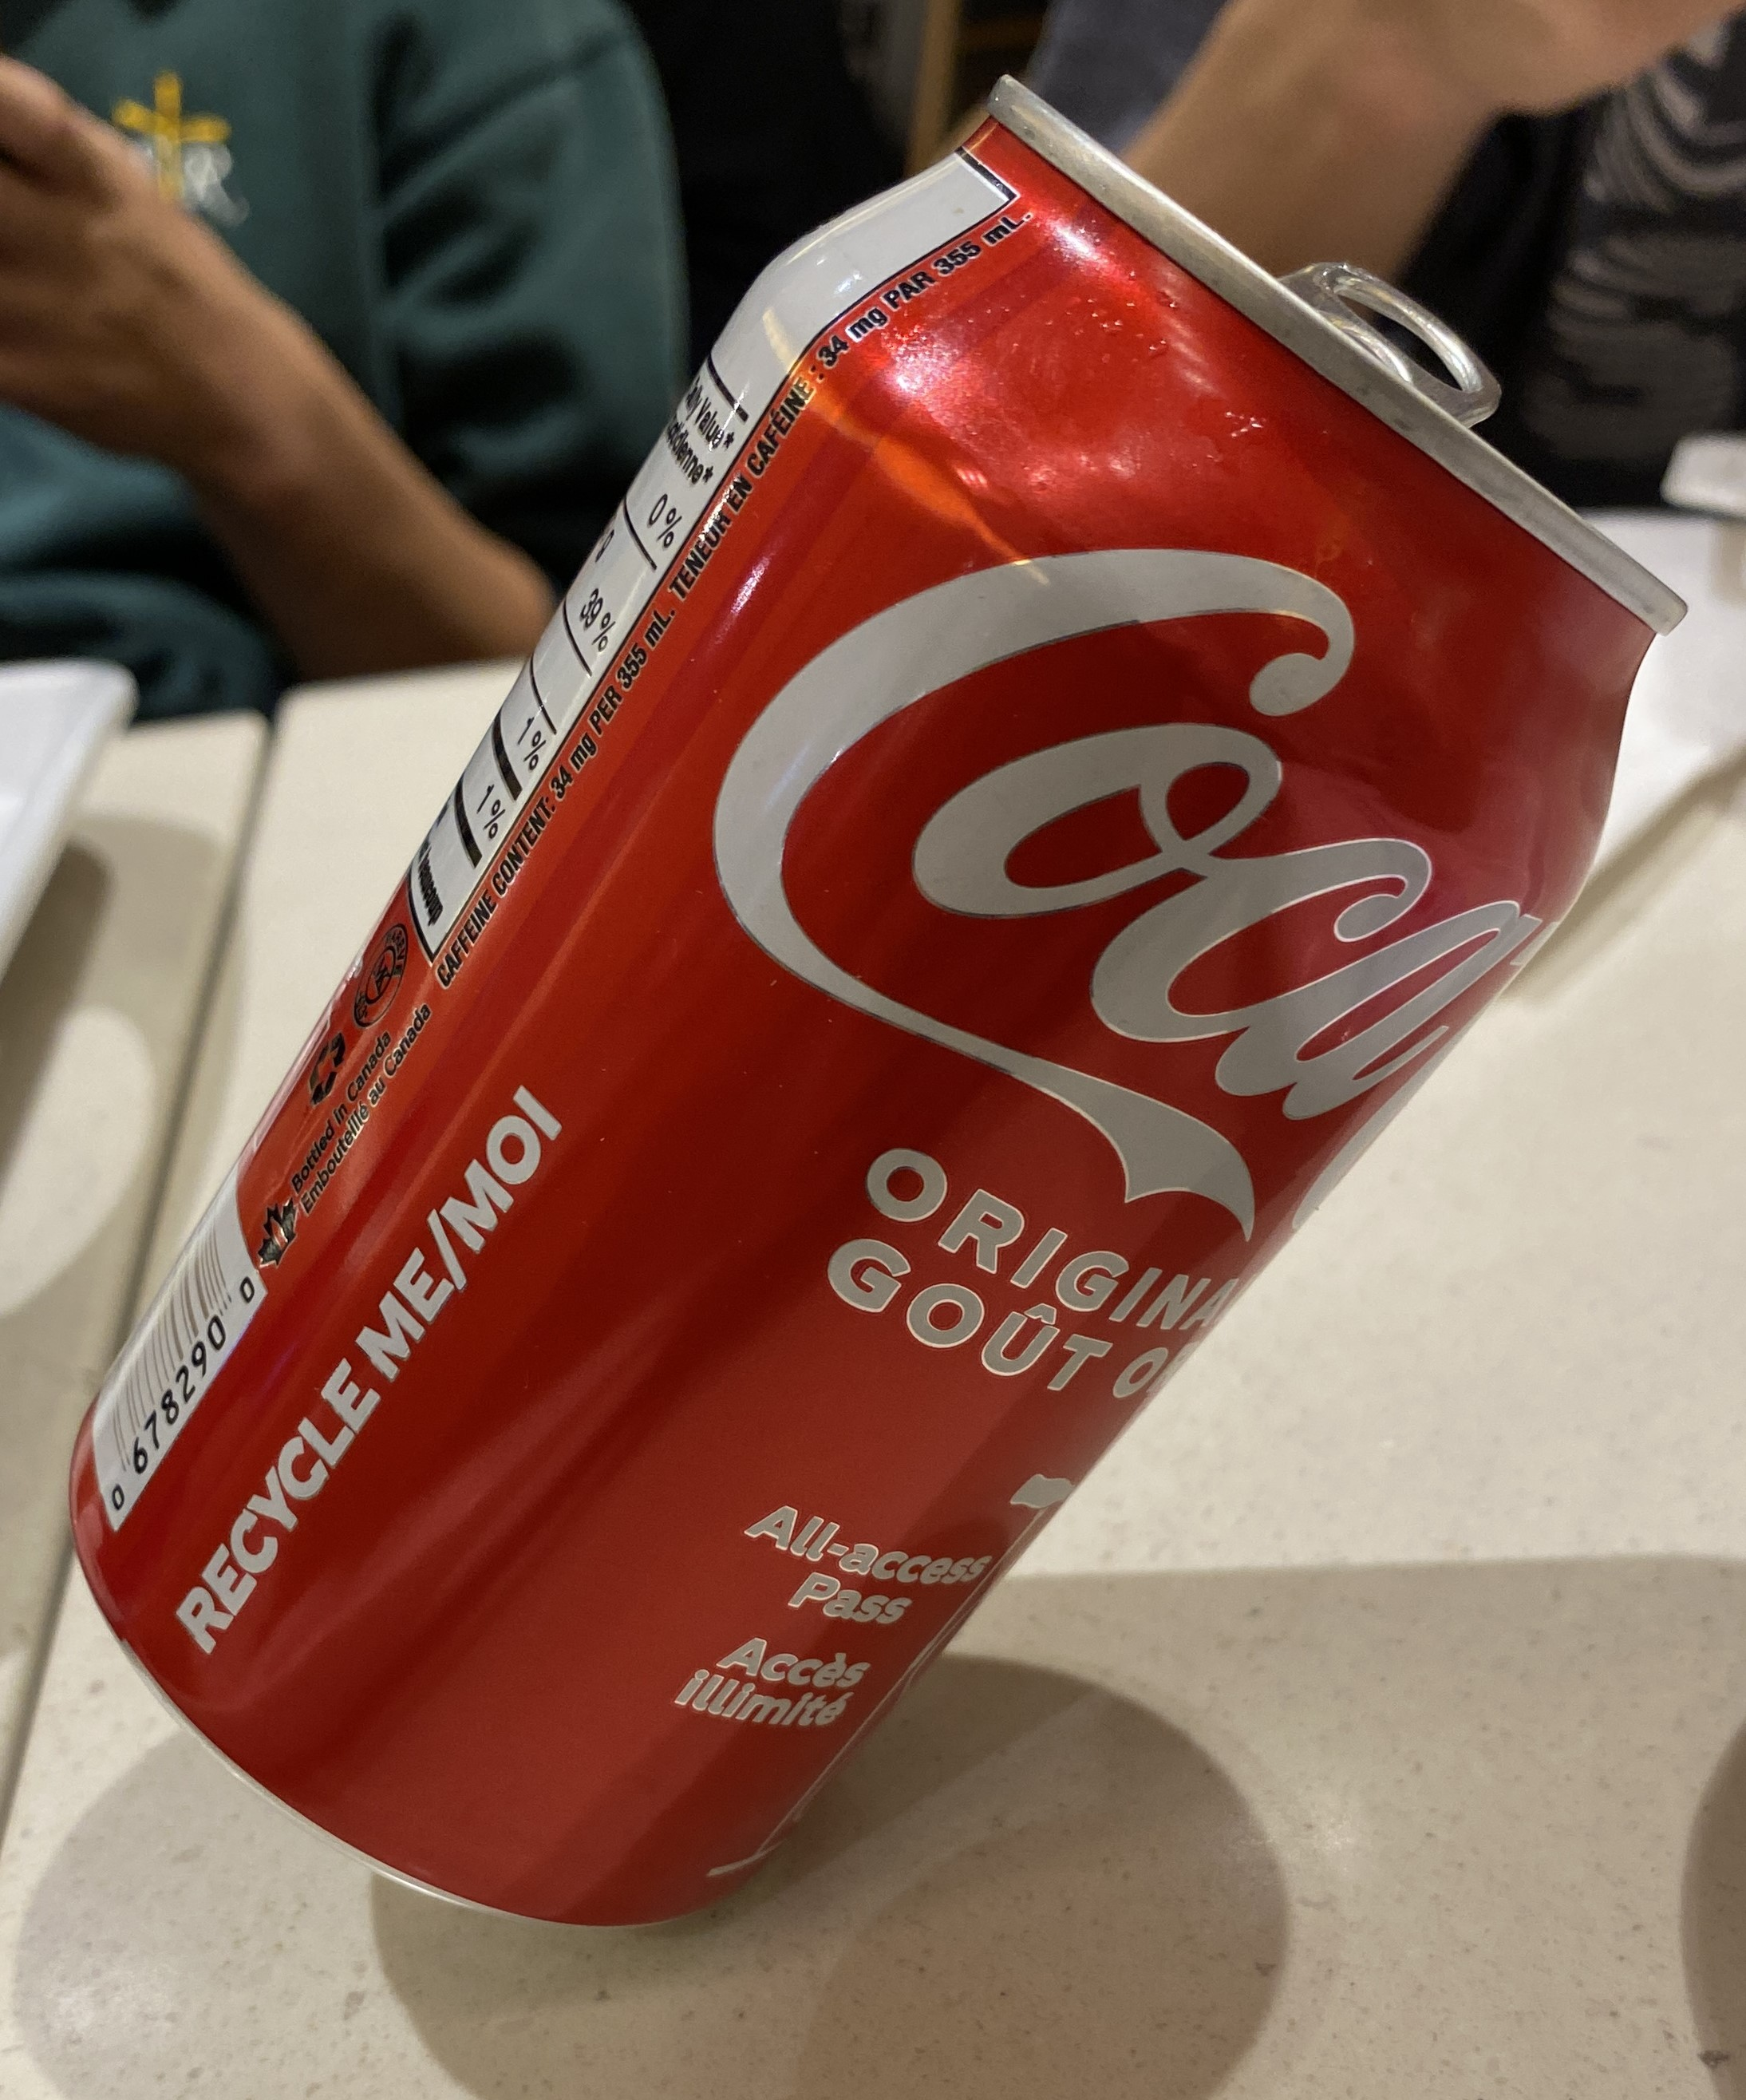
\includegraphics[width=.8\linewidth]{images/demonstration.jpg}
        \vspace{-10pt}
        \caption{Coke can balance on its edge}
        \label{fig:demo-image}
    \end{wrapfigure}

    If there is one thing in the world in which we should trust the most, it is our own intuition. But as we have all learned from various experiences, our intuitions can every so often lie to us. Personally, one of such occurrences came to me in the form of a demonstration I saw of someone setting a Coke can on its edge. Contrary to my immediate belief of the can being unstable without any support and sure to tip over, it actually stood perfectly balanced (Figure \ref{fig:demo-image}). I later learned that such a trick can be accomplished by filling up the empty can with just the right amount of water to counterbalance the weight of the can itself. Therefore, the aim of my exploration is to find the exact volumes of water that will make a standard $355 \mathrm{mL}$ aluminum Coke (or any other pop) can be able to be balanced on its edge. In order to do this, I will derive a function for the can's center of mass in terms of how much water is in it, using various integration techniques, followed by solving for the specific volumes of water so the entire system's center of mass is above a point where the can touches the floor.

    Recently in physics class we learned about center of mass (CM), a point in $3$D space where an object's weighted position is $0$. In other words, an object is balanced if its CM is directly above the point where the object touches the ground. The CM of an object can be decomposed into $\overline{x}$, $\overline{y}$ and $\overline{z}$, its CMs in the $x$, $y$ and $z$ directions, respectively. It is important to note that the CM of a system is independent of its orientation (Moore). That is, given the shape of an object remains the same, the CM stays the same even if it is tilted or upside down. For a uniformly dense object, its CM lies at its centroid, and this point can be found using two main equations, shown below (Moore). Both of which are listed for the $x$ axis, but analogous equations also exist for the $y$ and $z$ axes. The first of which is equation \eqref{eq:CM-sum} which works by splitting up an object into $N$ smaller objects. Variable $\overline{x_i}$ is the CM of the $i$-th object from the origin, $V_i$ the volume of the $i$-th object, and $V$ the total volume of the system. The second equation is \eqref{eq:CM-integral}, which is equation \eqref{eq:CM-sum} in integral form. In this case, $dV$ is the volume of an infinitely thin cross-sectional slice of the object (Figure \ref{fig:volume-crosssection}), $x$ is the position of that thin slice, and $V$ is still the total volume. In the case that different parts of a system are of different densities, formula \eqref{eq:CM-density} can be used, where $\rho_i$ is the density of the $i$-th object, and $\overline{x}_i$ is the CM of the $i$-th object and $V_i$ the volume of the $i$-th object. Finally, if an object is symmetrical along a plane, its CM lies on that plane (Isaac Physics).

    \begin{minipage}{.4\textwidth}
        \begin{figure}[H]
            \centering
            \frame{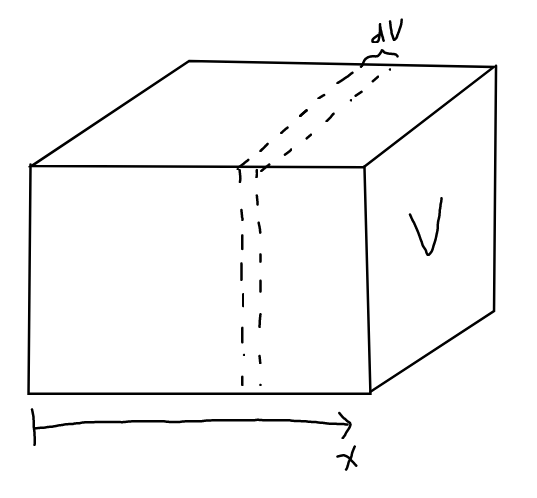
\includegraphics[width=.7\linewidth]{images/volume_crosssection.png}}
            \vspace{-10pt}
            \caption{Cross-sectional volume}
            \label{fig:volume-crosssection}
        \end{figure}
    \end{minipage}%
    \begin{minipage}{.6\textwidth}
        \begin{align*}
            \overline{x} &= \frac{\sum_{i=1}^N \overline{x_i} V_i}{V} \numberthis{\label{eq:CM-sum}} \\
            \overline{x} &= \frac{\int x dV}{V} \numberthis{\label{eq:CM-integral}} \\
            \overline{x} &= \frac{\sum_{i=1}^N \overline{x_i} \rho_i V_i}{\sum_{i=1}^N \rho_i V_i} \numberthis{\label{eq:CM-density}}
        \end{align*}
    \end{minipage}
    \vspace{6pt}

    \begin{wrapfigure}[8]{r}{.5\textwidth}
        \centering
        \frame{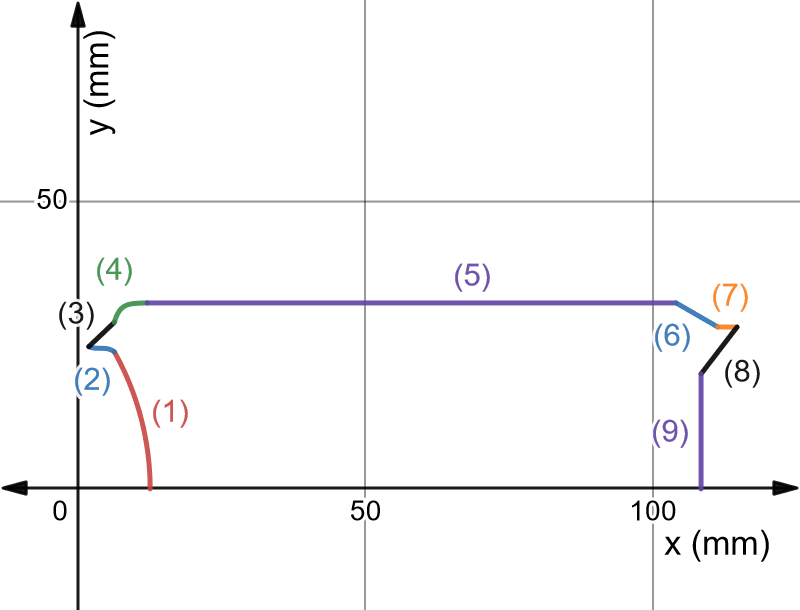
\includegraphics[width=.9\linewidth]{images/can_model.png}}
        \vspace{-10pt}
        \caption{Model of the can in Desmos}
        \label{fig:desmos-model}
    \end{wrapfigure}

    I first modelled the inner walls of the can in Desmos with a scale of $1$ unit on the graph being equal to $1 \mathrm{mm}$ in real life (Figure \ref{fig:desmos-model}). I tilted the can on its side, so I could express the functions that model the can as functions of $x$ and not $y$, for the purpose of simplicity. The dimensions of the main body of a can and the reference cross-sectional image of the can are sourced from an aluminum can manufacturer's website (Helvetia Packaging), as I did not have the tools to cut a can in half safely. The top part of the can, referred to as a ``can end'' is sourced from a separate manufacturer's website (Can Ends). The pop tab at the top of the can was not modelled as its mass is too small to make a significant difference on the CM of the can, weighing in at only $0.3 \mathrm{g}$ compared to the approximate $80 \mathrm{g}$ weight of a balancing can (Mulkins). An important value for the model is the can's out-most wall's radius, $R = 32.35 \mathrm{mm}$. The modelling was done using various functions, each of which alongside its domain and why I chose it are listed in Table \ref{tab:functions}. Note that the distance from the $x$-axis to $f_5(x)$ is equal to $R$, so $f_5(x)$ also equals the radius of the can.
    \begin{table}[H]
        \scriptsize
        \renewcommand{\arraystretch}{0.9}
        \centering
        \caption{List of functions used to model the can}
        \vspace{-8pt}
        \begin{tabularx}{\textwidth}{|l|l|l|X|}
            \hline
            $i$ & Domain & $f_i(x)$ & Rationale \\
            \hline \hline
            $1$ & $6.26 \le x \le 12.5$ & $\sqrt{(48.7)^2 - (x + 36.2)^2}$ & An equation for a circle with radius $48.7$ centered at $(0,-36.2)$ rearranged to be a function of $x$, in order to fit the rounded bottom of the can. \\
            \hline
            $2$ & $1.81 \le x \le 6.26$ & $-0.039x^3 + 0.44x^2 - 1.64x + 26.5$ & I chose $4$ points on the image of the can and solved for a cubic polynomial that fit them. \\
            \hline
            $3$ & $1.81 \le x \le 6.26$ & $0.944x + 23$ & I saw that this part of the can was flat, so I solved for a straight line using $2$ points on the image. \\
            \hline
            $4$ & $6.26 \le x \le 12$ & $-\frac{e^{-x}}{0.000564} + 32.4$ & The main body of the can had a small curve at the bottom and was straight until the top, which I knew fit the characteristics of an inverse exponential function. I plotted $2$ points on the image and used them to solve for the variables $d$ and $c$ in $y = \frac{e^{-x}}{d} + c$. \\
            \hline
            $5$ & $12 \le x \le 104$ & $32.35$ & This is the outer wall for the majority of the can, which is flat and therefore modelled as a horizontal line. \\
            \hline
            $6$ & $104 \le x \le 111.25$ & $-0.578x + 92.45$ & Same as equation $3$. \\
            \hline
            $7$ & $111.25 \le x \le 114.6$ & $28.16$ & Same as equation $3$. \\
            \hline
            $8$ & $108.34 \le x \le 114.6$ & $1.304x - 121.22$ & Same as equation $3$ \\
            \hline
            $9$ & $108.34 \le x \le 108.4$ & $-333.333x + 36133.33$ & Same as equation $3$, but instead of having a vertical line, I gave it a defined slope to be able to integrate in terms of $x$. \\
            \hline
        \end{tabularx}
        \label{tab:functions}
    \end{table}
    \vspace{-10pt}

    After modelling the can, I can move on to find the CM of the can with water inside. Water and aluminum are by themselves of uniform density. However, the two densities are different and therefore equations \eqref{eq:CM-sum} and \eqref{eq:CM-integral} do not hold for the combined system. Hence, I had to split up the can with water into two parts: the empty can and the water inside without the can. By finding the CMs of the can and water separately, I can combine them afterwards using equation \eqref{eq:CM-density} to find the entire system's CM.

    \begin{wrapfigure}[5]{r}{.55\textwidth}
        \centering
        \frame{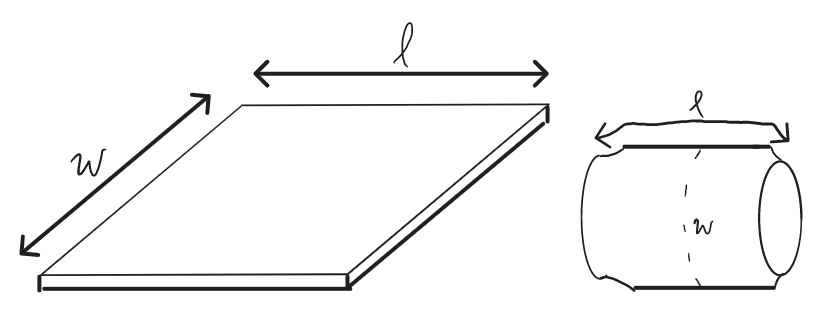
\includegraphics[width=.9\linewidth]{images/aluminum_sheet.png}}
        \vspace{-10pt}
        \caption{Rolled up aluminum sheet}
        \label{fig:aluminum-sheet}
    \end{wrapfigure}

    I started off by finding the CM of the empty can. The can itself is symmetrical along both the $y$ and $z$ axes, so $\overline{y} = 0$ and $\overline{z} = 0$. All that needs to be solved for is $\overline{x}$. The manufacturing process of an aluminum can involves rolling and forming a thin aluminum sheet of constant thickness $T$ into a can shape. This process causes different parts of the can's walls to be disproportionately compressed. Therefore, it would be impractical to try and accurately solve for the volume of the can using solids of revolution. Alternatively, I made the observation that the unrolled aluminum sheet has equal volume to the can. When rolled, the width of the sheet, $w$, becomes the circumference of the can, while the length, $l$, becomes the cumulative length down the height of the can (Figure \ref{fig:aluminum-sheet}). By splitting the can into infinitely thin slices down its length, each of length $dl$, each slice can be ``unrolled'' back into a slice of the original aluminum sheet. The unrolled slice is a rectangular prism of width $w$, length $dl$ and height or thickness $T$. Therefore, the slice's volume is $dV = wT \, dl$. When the sheet is rolled into a cylindrical shape, its radius is equal to a function $f(x)$ which represents the can's radius at a distance $x$ from the origin. Therefore, the circumference of the can, which is equal to $w$, is $2 \pi f(x)$. For the purpose of convention, $dl$ is renamed to $ds$. Altogether, the slice's volume is $dV = 2 \pi T f(x) \, ds$ (Figure \ref{fig:can-slice}). Furthermore, for certain parts of the can, several layers of the sheet metal are used to enhance its structural integrity. For example, the top and bottom of a can are slightly thicker than its walls. Consequently, the bottom is $0.3 \mathrm{mm}$ thick, the walls $0.11 \mathrm{mm}$, and the top $0.16 \mathrm{mm}$ (Talat).

    \begin{figure}[H]
        \centering
        \begin{minipage}{.5\textwidth}
            \centering
            \frame{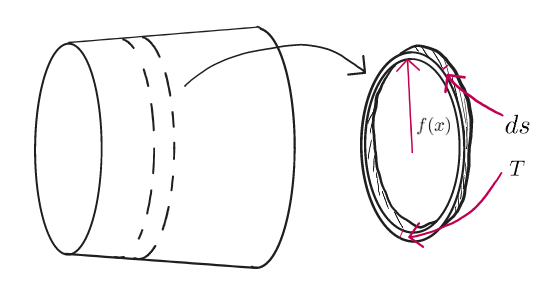
\includegraphics[width=.8\linewidth]{images/can_slices.png}}
            \vspace{-10pt}
            \caption{A cross-sectional slice of the can}
            \label{fig:can-slice}
        \end{minipage}%
        \begin{minipage}{0.5\textwidth}
            \centering
            \frame{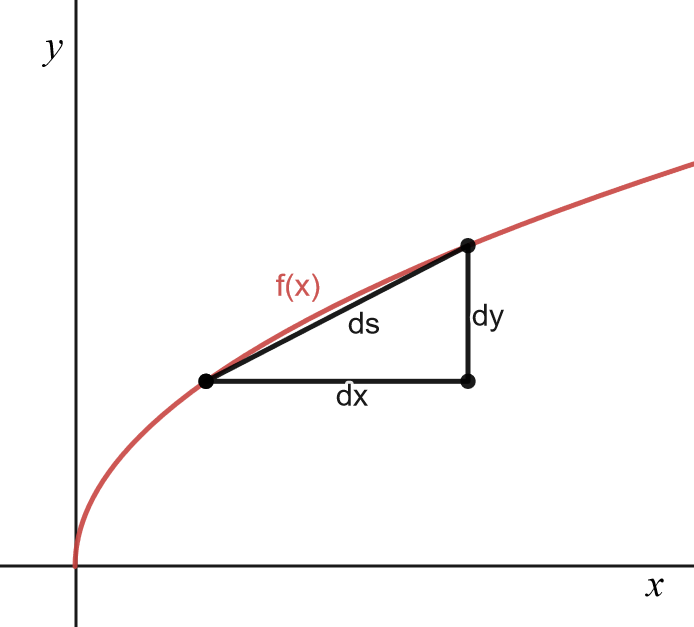
\includegraphics[width=.5\linewidth]{images/arc_length.png}}
            \vspace{-10pt}
            \caption{Length of an infinitely small segment}
            \label{fig:arc-length}
        \end{minipage}
    \end{figure}
    \vspace{-10pt}

    \begin{wrapfigure}{r}{.35\linewidth}
        {\footnotesize\begin{align*}
            (ds)^2 &= (dx)^2 + (dy)^2 \\
            ds &= \sqrt{(dx)^2 + (dy)^2} \\
            &= \sqrt{(dx)^2 \left( 1 + \frac{(dy)^2}{(dx)^2} \right)} \\
            &= \sqrt{1 + \left( \frac{dy}{dx} \right)^2} \, dx \\
            ds &= \sqrt{1 + (f'(x))^2} \, dx
        \end{align*}}
    \end{wrapfigure}

    The value of $ds$ is the instantaneous arc length of the walls of the can, and can be derived using Pythagorean's Theorem. The value of each $ds$ is the hypotenuse of a triangle with base $dx$ and height $dy$ (Figure \ref{fig:arc-length}), so $(ds)^2 = (dx)^2 + (dy)^2$. This can be rearranged, as shown on the right.

    Substituting the value of $ds$ into the equation for a cross-sectional slice's volume gives $dV = 2 \pi T f(x) \sqrt{1 + (f'(x))^2} \, dx$.

    \begin{wrapfigure}{r}{.4\textwidth}
        \footnotesize
        \begin{align*}
            \overline{x_i} &= \frac{\int_{a_i}^{b_i} x dV}{V_i} \\
            &= \frac{\int_{a_i}^{b_i} x 2 \pi T f_i(x) \sqrt{1 + (f_i'(x))^2} \, dx}{V_i} \\
            \overline{x_i} &= \frac{2 \pi T \int_{a_i}^{b_i} x f_i(x) \sqrt{1 + (f_i'(x))^2} \, dx}{V_i}
        \end{align*}
    \end{wrapfigure}

    Next, the can is split up into various sections based on the function that models each range of $x$ values. The volume of the part of the can modelled by function $f_i(x)$ is given by $V_i = \int_{a_i}^{b_i} dV$, where $a_i$ and $b_i$ are the upper and lower limits of the function's domain, respectively. I substituted this equation and the value of $dV$ into formula \eqref{eq:CM-integral} to find $\overline{x_i}$, shown on the right. This equation is in turn substituted into \eqref{eq:CM-sum}, with $N = 9$, the number of functions used to model the can.

    \begin{minipage}{.55\textwidth}
        \footnotesize
        \begin{align*}
            \overline{x} &= \frac{\sum_{i=1}^9 \overline{x_i} V_i}{V} \\[5pt]
            &= \frac{\sum_{i=1}^9 \overline{x_i} V_i}{\sum_{i=1}^9 V_i} \\[5pt]
            &= \frac{\sum_{i=1}^9 \left( \frac{2 \pi T_i \int_{a_i}^{b_i} x f_i(x) \sqrt{1 + (f_i'(x))^2} \, dx}{V_i} \right) \cdot V_i}{\sum_{i=1}^9 \left( \int_{a_i}^{b_i} dV \right)} \\[5pt]
            &= \frac{\sum_{i=1}^9 2 \pi T_i \int_{a_i}^{b_i} x f_i(x) \sqrt{1 + (f_i'(x))^2} \, dx}{\sum_{i=1}^9 \left( \int_{a_i}^{b_i} 2 \pi T_i f(x) \sqrt{1 + (f'(x))^2} \, dx \right)} \\[5pt]
            &= \frac{2 \pi \sum_{i=1}^9 T_i \int_{a_i}^{b_i} x f_i(x) \sqrt{1 + (f_i'(x))^2} \, dx}{2 \pi \sum_{i=1}^9 T_i \int_{a_i}^{b_i} f_i(x) \sqrt{1 + (f_i'(x))^2} \, dx} \numberthis{\label{eq:can-x-frac}} \\[5pt]
            &= \frac{\sum_{i=1}^9 T_i \int_{a_i}^{b_i} x f_i(x) \sqrt{1 + (f_i'(x))^2} \, dx}{\sum_{i=1}^9 T_i \int_{a_i}^{b_i} f_i(x) \sqrt{1 + (f_i'(x))^2} \, dx} \\[5pt]
            \overline{x} &= \frac{\sum_{i=1}^9 T_i A_i}{\sum_{i=1}^9 T_i B_i} \numberthis{\label{eq:can-x-cm}}
        \end{align*}
    \end{minipage}%
    \begin{minipage}{.45\textwidth}
        \footnotesize
        \centering
        \vspace{170pt}
        Where:
        \begin{align*}
            A_i &= \int_{a_i}^{b_i} x f_i(x) \sqrt{1 + (f_i'(x))^2} \, dx \\[5pt]
            B_i &= \int_{a_i}^{b_i} f_i(x) \sqrt{1 + (f_i'(x))^2} \, dx
        \end{align*}
        $T_i$ is the thickness of the $i$-th portion of the can.
    \end{minipage}
    \vspace{4pt}

    The bottom of the can consists of functions $f_1$ through $f_4$, the walls functions $f_5$ and $f_6$, and the top functions $f_7$ through $f_9$. Using Desmos, I found the values of $A_i$ and $B_i$ for each function $f_i(x)$, and listed them alongside each $T_i$ in Table \ref{tab:can-x-integrals}. The values are all rounded to $2$ decimal places, which is reasonable as any more decimals would be less than $0.01 \mathrm{mm}$, and beyond conceivable accuracy. This pattern will continue for the rest of the exploration.

    \begin{table}[H]
        \scriptsize
        \renewcommand{\arraystretch}{0.9}
        \centering
        \caption{Values needed in finding $\overline{x}$ of the empty can}
        \vspace{-8pt}
        \begin{tabular}{|c|c|c|c|}
            \hline
             $i$ & $A_i$ & $B_i$ & $T_i$ \\
             \hline \hline
             $1$ & $2850.47$ & $303.89$ & $0.3$ \\
             \hline
             $2$ & $456.17$ & $112.38$ & $0.3$ \\
             \hline
             $3$ & $671.52$ & $164.06$ & $0.3$ \\
             \hline
             $4$ & $2031.51$ & $234.60$ & $0.3$ \\
             \hline
             $5$ & $172619.60$ & $2976.20$ & $0.11$ \\
             \hline
             $6$ & $27234.92$ & $253.25$ & $0.11$ \\
             \hline
             $7$ & $10652.89$ & $94.34$ & $0.16$ \\
             \hline
             $8$ & $27721.43$ & $248.30$ & $0.16$ \\
             \hline
             $9$ & $22447.59$ & $207.16$ & $0.16$ \\
             \hline
        \end{tabular}
        \label{tab:can-x-integrals}
    \end{table}
    \vspace{-10pt}

    Combining these values into \eqref{eq:can-x-cm} yields the overall $\overline{x}$ of the can. I split up the summation into $3$ parts according to each of the $3$ different parts of the can with different thicknesses. The values of $T_1$ through $T_4$ are all the same, and therefore are combined into just $T_1$ for simplicity. The same was done for $T_5$ through $T_6$ and $T_7$ through $T_9$.
    {\footnotesize\begin{align*}
        \overline{x} &= \frac{\sum_{i=1}^9 T_i A_i}{\sum_{i=1}^9 T_i B_i} \\
        \overline{x} &= \frac{T_1 \sum_{i=1}^4 A_i + T_5 \sum_{i=5}^6 A_i + T_7 \sum_{i=7}^9 A_i}{T_1 \sum_{i=1}^4 B_i + T_5 \sum_{i=5}^6 B_i + T_7 \sum_{i=7}^9 B_i}
    \end{align*}}

    Each of the $3$ summations multiplied by their $T$ values in the numerator and denominator are calculated individually, as show below:

    \begin{minipage}{.45\linewidth}
        {\footnotesize\begin{align*}
            T_1 \sum_{i=1}^4 A_i &= 0.3(2850.47 + 456.17 + 671.52 + 2031.51) = 1802.90 \\
            T_5 \sum_{i=5}^6 A_i &= 0.11(172619.60 + 27234.92) = 21984.00 \\
            T_7 \sum_{i=7}^9 A_i &= 0.16(10652.89 + 27721.43 + 22447.59) = 9731.51 \\
            T_1 \sum_{i=1}^4 B_i &= 0.3(303.89 + 112.38 + 164.06 + 234.60) = 244.48 \\
            T_5 \sum_{i=5}^6 B_i &= 0.11(2976.20 + 253.25) = 355.24 \\
            T_7 \sum_{i=7}^9 B_i &= 0.16(94.34 + 248.30 + 207.16) = 87.97
        \end{align*}}
    \end{minipage}%
    \begin{minipage}{.4\linewidth}
        \vspace{60pt}
        These values are recombined to find the overall $\overline{x}$.
        {\footnotesize\begin{align*}
            \overline{x} &= \frac{1802.90 + 21984.00 + 9731.51}{244.48 + 355.24 + 87.97} \\
            &= \frac{33518.41}{687.69} \\
            \overline{x} &= 48.74 \mathrm{mm}
        \end{align*}}
    \end{minipage}
    \vspace{16pt}

    The CM of the empty can along its $x$-axis is at $48.74 \mathrm{mm}$. The height of the can is $115.2 \mathrm{mm}$ (Helvetia Packaging). Thus, the value of this CM makes sense as it is almost half of the height, and a bit lower due to the thicker, and therefore ``heavier'', bottom of the can. Next, I noticed that the volume of the aluminum in the can is in fact the denominator of the right-hand side in equation \eqref{eq:can-x-frac}. After rearranging and substituting in values, $V_{can}$ is calculated to be:

    \begin{minipage}{.6\linewidth}
        \footnotesize
        \begin{align*}
            V_{can} &= 2 \pi \sum_{i=1}^9 \left( T_i \int_{a_i}^{b_i} f_i(x) \sqrt{1 + (f_i'(x))^2} \, dx \right) \\
            &= 2 \pi \sum_{i=1}^9 T_i B_i \\
            &= 2 \pi \left( T_1 \sum_{i=1}^4 B_i + T_5 \sum_{i=5}^6 B_i + T_7 \sum_{i=7}^9 B_i \right) \\
            &= 2 \pi \cdot (244.48 + 355.24 + 87.97) \\
            V_{can} &= 4320.88 \mathrm{mm}^3
        \end{align*}
    \end{minipage}%
    \begin{minipage}{.4\linewidth}
        \begin{figure}[H]
            \centering
            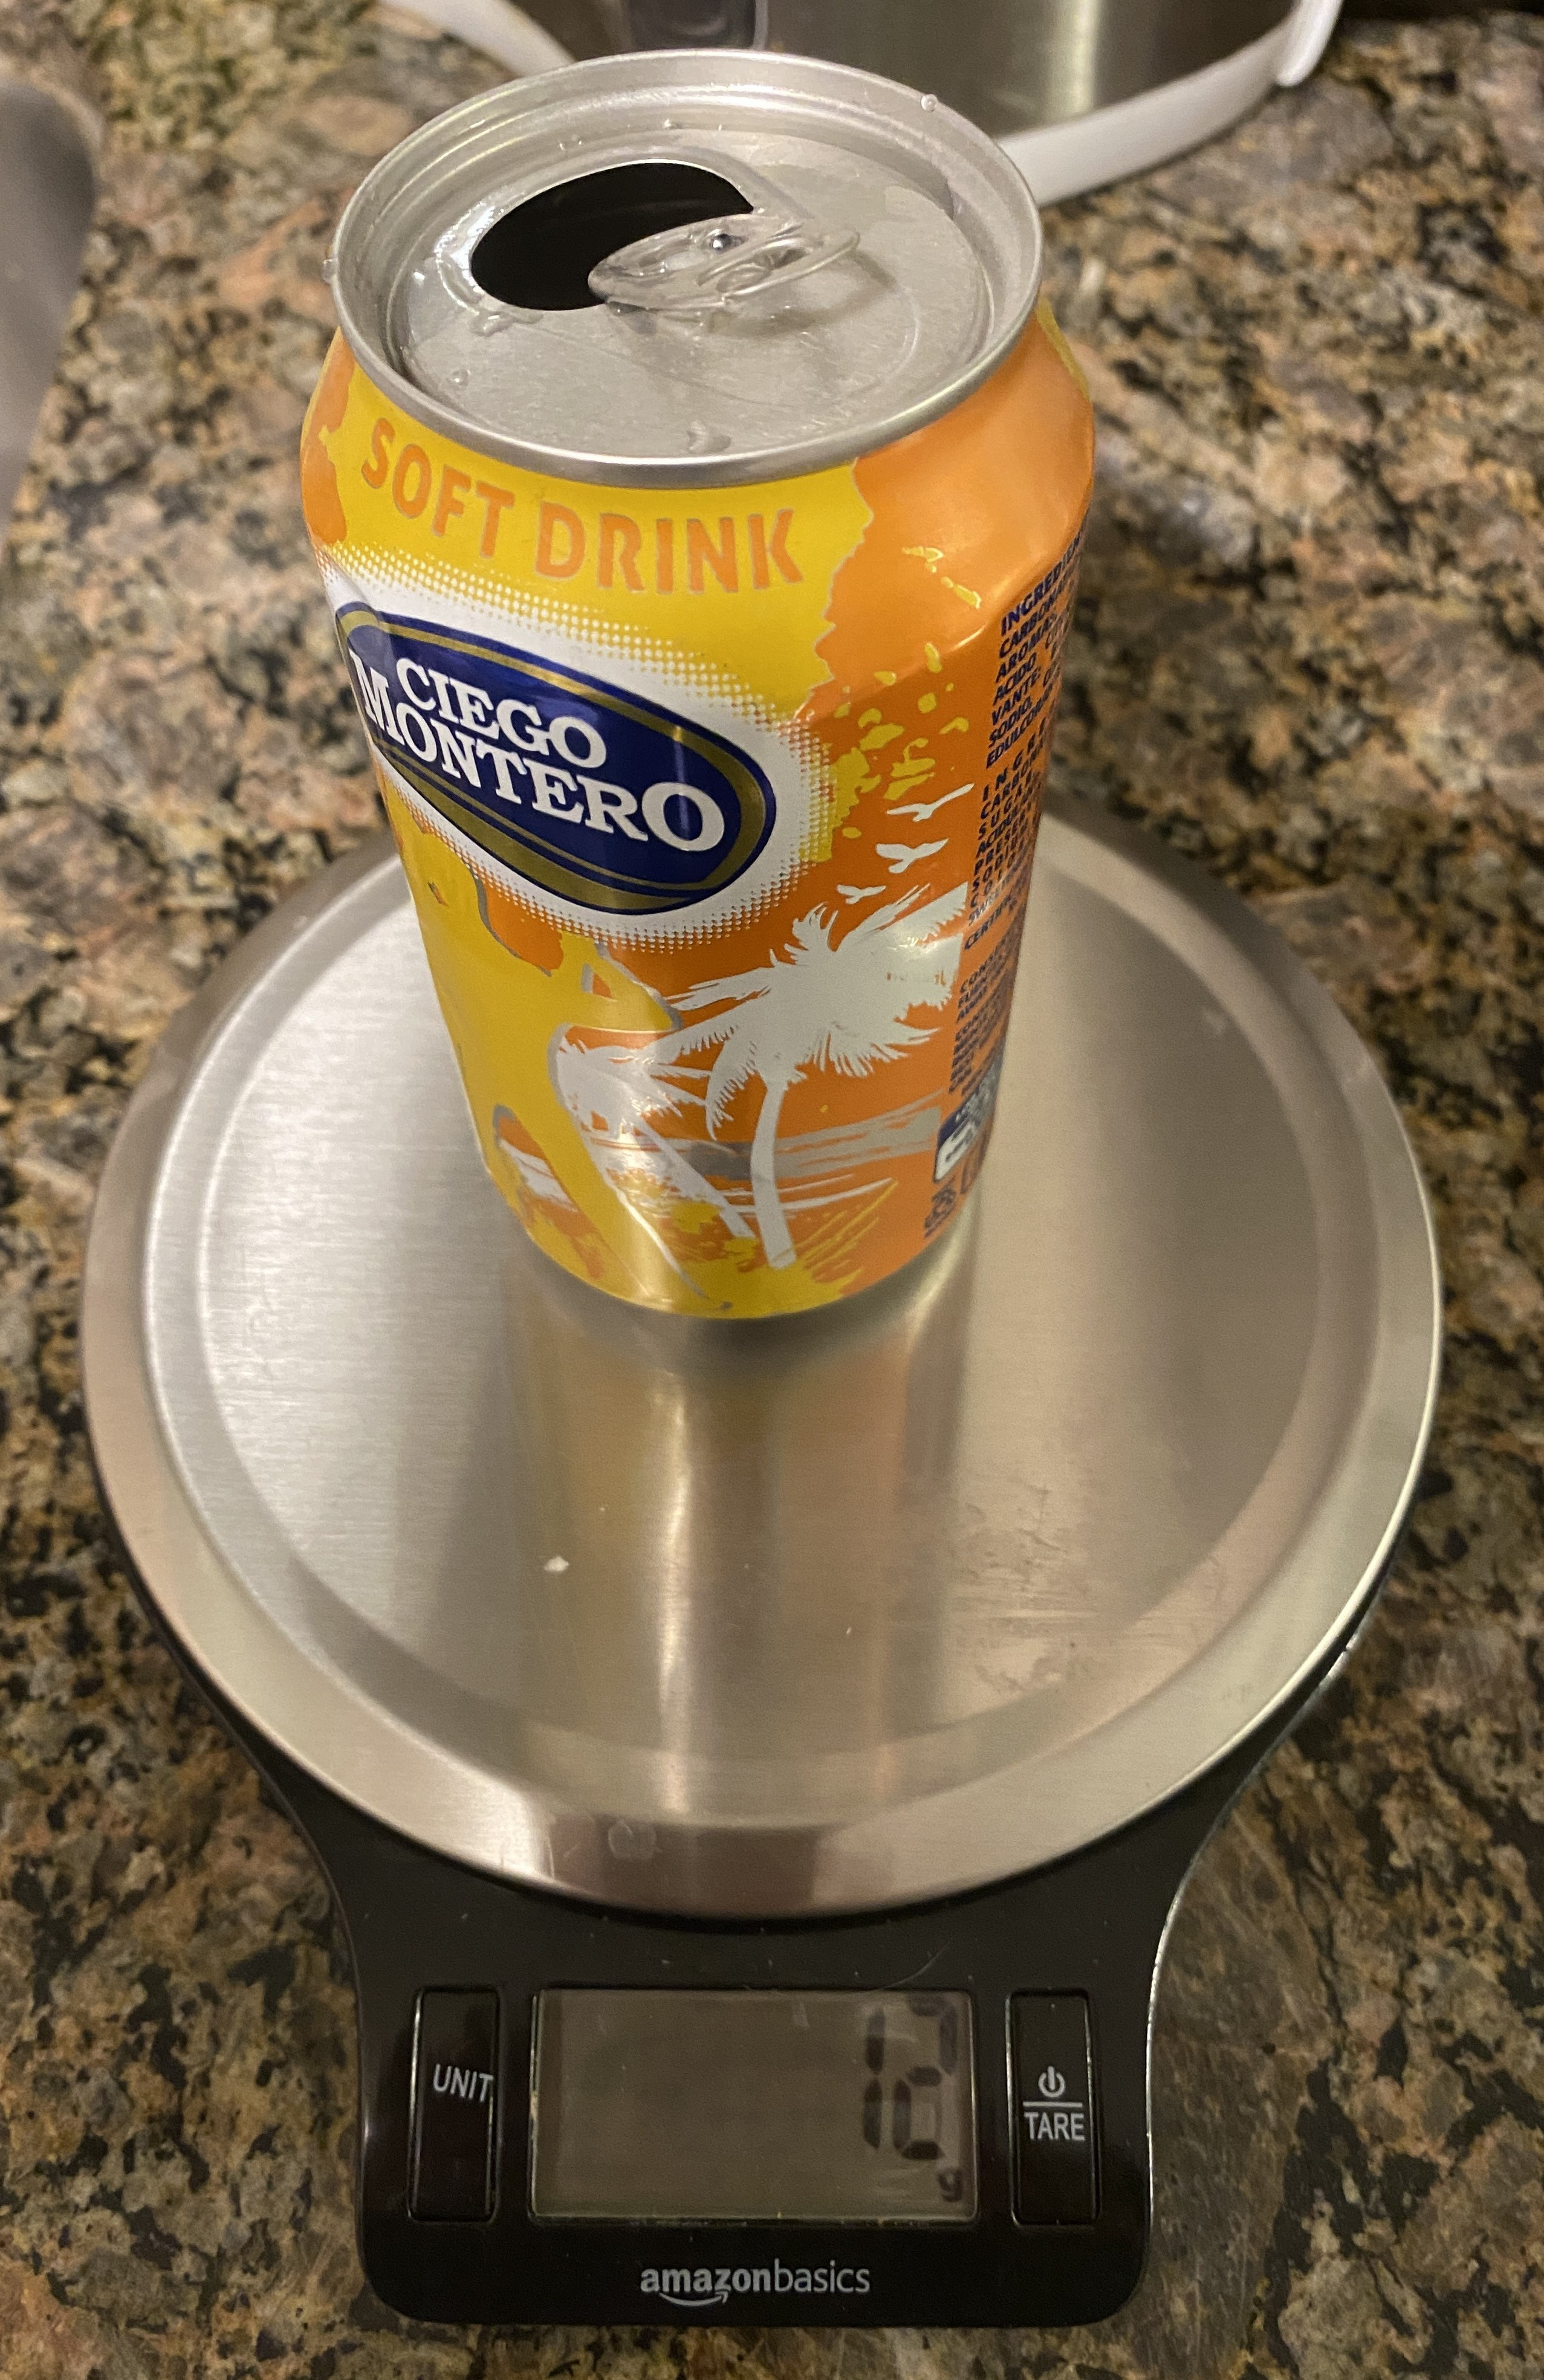
\includegraphics[width=.7\linewidth]{images/scale_12.JPG}
            \vspace{-10pt}
            \caption{Mass of empty can}
            \label{fig:scale-12}
        \end{figure}
    \end{minipage}
    \vspace{4pt}

    In order to validate the value of $V_{can}$, I used the formula to convert volume to mass, $m = \rho V$, where $\rho$ is the density of aluminum, $\rho = 0.0027 \frac{\mathrm{g}}{\mathrm{mm}^3}$. Therefore, $m_{can} = 0.0027 \frac{\mathrm{g}}{\mathrm{mm}^3} \cdot 4320.88 \mathrm{mm}^3 \approx 11.7 \mathrm{g}$. Measuring an empty aluminum can on a scale gave me $12 \mathrm{g}$ (Figure \ref{fig:scale-12}), which is very close to the calculated mass. Thus, my calculations are accurate.

    % TODO: maybe make this image a bit wider
    \begin{wrapfigure}[10]{l}{.45\textwidth}
        \centering
        \frame{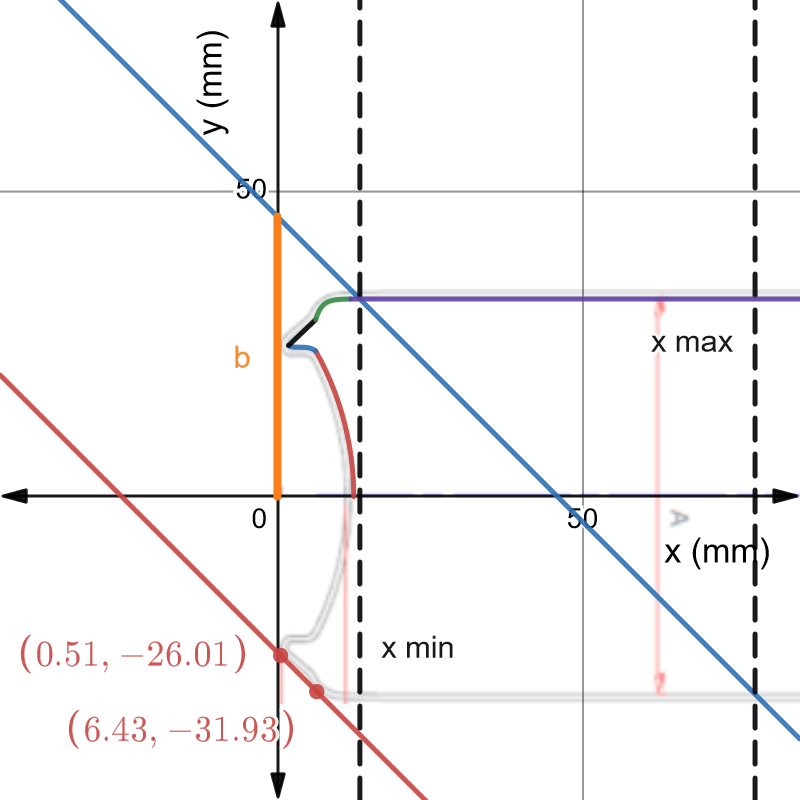
\includegraphics[width=.8\linewidth]{images/floor_and_water.png}}
        \vspace{-10pt}
        \caption{The floor and surface of the water}
        \label{fig:floor}
    \end{wrapfigure}

    The next step is to find the CM of the water using integration. When the can is tilted at an angle, the surface of the water will be parallel to the floor, hence the lines that model the floor and water have the same slope. I first plotted two points on the bottom edge of the can, where it would be touching the floor, at $(6.43, -31.93)$ and $(0.51, -26.01)$, and found the slope using $m = \frac{\Delta y}{\Delta x} = -1$ (Figure \ref{fig:floor}). The equation that models the surface of the water is $f_{water}(x) = -x + b$, where $b$ is a constant that correlates to how much water is in the can. This function is visualized by the blue line in Figure \ref{fig:floor}. I further split up the water into two sections based on the $x$ value of where the lower end of the water surface meets the inner wall of the can, visualized by the dashed line labelled ``$x$ min'' in Figure \ref{fig:floor}. This was done as integrating the two parts separately would be much easier than trying to do them together. The $x$ values of where the water line intersect the outer walls of the can be solved by setting $f_{water}(x) = \pm f_5(x)$:
    {\footnotesize\begin{align*}
        f_{water}(x) &= \pm f_5(x) \\
        -x + b &= \pm 32.35 \\
        x &= b \mp 32.35 \\
        x_{min} &= b - 32.35 \\
        x_{max} &= b + 32.35
    \end{align*}}

    Therefore, the domain of $f_{water}(x)$ is $\{ x \in \mathbb{R} \, | \, x_{min} \le x \le x_{max} \}$, as water can not go through the solid walls of the can. The bottom (left of the dotted line on Figure \ref{fig:floor}) of the can covers the volume for which ${x \le x_{min}}$ and the top of the can covers the volume for which ${x_{min} \le x \le x_{max}}$. Note that
    \begin{wrapfigure}{r}{.23\linewidth}
        \vspace{-10pt}
        {\footnotesize\begin{align*}
            x_{min} &\ge 12.5 \\
            b - 32.35 &\ge 12.5 \\
            b &\ge 44.85
        \end{align*}}
    \end{wrapfigure}
    these two values can also be rewritten in terms of $R$, as $x_{min} = b - R$ and $x_{max} = b + R$. In order to simplify calculations and be able to use solid of revolution for the bottom of the can, a limitation was put in place so that $x_{min}$ does not intersect with the indent at the bottom of the can. In other words, $x_{min} \ge 12.5$. This inequality can be rearranged in terms of $b$, shown to the right.

    \begin{wrapfigure}[9]{r}{.5\textwidth}
        \centering
        \frame{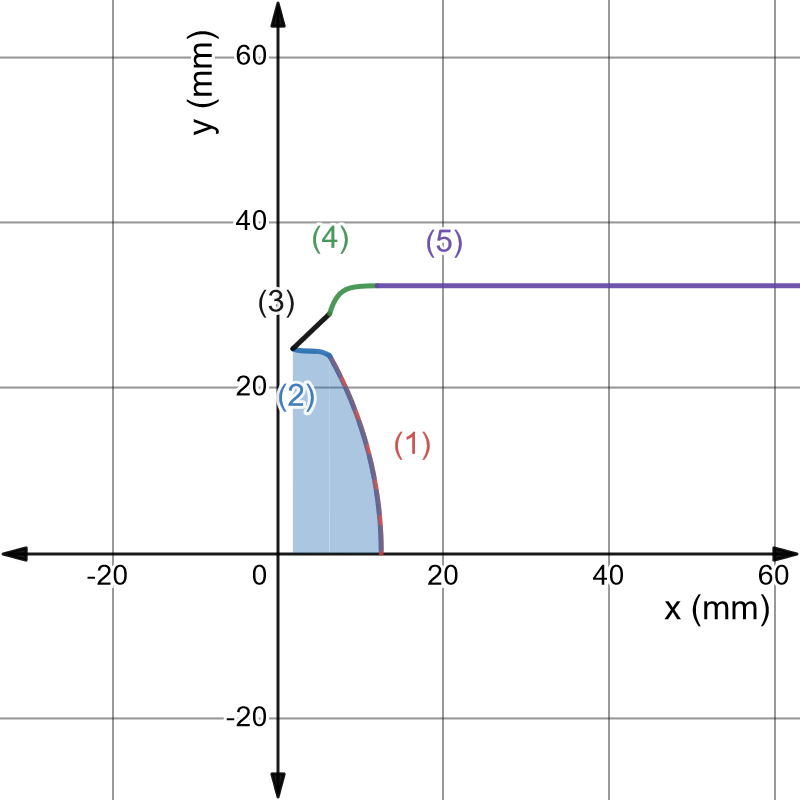
\includegraphics[width=.8\linewidth]{images/negative_area.png}}
        \vspace{-10pt}
        \caption{The area under $f_1(x)$ and $f_2(x)$ is negative}
        \label{fig:negative-area}
    \end{wrapfigure}

    The first step is the part of the water at the bottom of the can, to the left of the line $x_{min}$ in Figure \ref{fig:floor}. Similar to the empty can, this portion of water has rotation symmetry along the $x$-axis, and therefore, has $\overline{y} = 0$ and $\overline{z} = 0$. All that needs to be solved for is $\overline{x}$. There is a ``dent'' at the bottom of a soda can, which takes away from its total volume, illustrated in Figure \ref{fig:negative-area} by the area highlighted in blue.

    \begin{wrapfigure}[7]{r}{.45\textwidth}
        \centering
        \frame{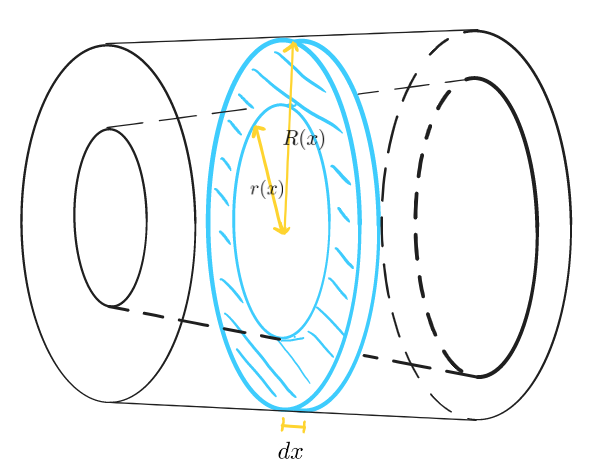
\includegraphics[width=.8\linewidth]{images/washer_method.png}}
        \vspace{-10pt}
        \caption{Washer method}
        \label{fig:washer-method}
    \end{wrapfigure}

    Therefore, the volume of the bottom portion of water in the can is the volume of the can minus the volume of the indented portion. Similar to the can, the volume of the water can be split up into the sum of an infinite number of circular cross-sections. Rather, in this case, the cross-sectional volumes are uniformly dense ``washers'', an outer disk minus the inner disk. The volume of the outer disk, $dV_R$, is the area of its base with radius $R(x)$ multiplied by its width $dx$, so $dV_R = \pi R(x)^2 \, dx$. Accordingly, the volume of the inner disk, $dV_r$, with radius $r(x)$ and the same width $dx$ is $dV_r = \pi r(x)^2 \, dx$. This technique is called the washer method, and is visualized by the shaded area in Figure \ref{fig:washer-method}. Combined, the volume of each cross-section is:

    \begin{minipage}{.5\linewidth}
        \footnotesize
        \begin{align*}
            dV &= dV_R - dV_r \\
            &= \pi R(x)^2 \, dx - \pi r(x)^2 \, dx \\
            dV &= \pi \left( R(x)^2 - r(x)^2 \right) \, dx
        \end{align*}
    \end{minipage}%
    \begin{minipage}{.5\linewidth}
        \vspace{20pt}
        Substituting this into equation \eqref{eq:CM-integral} gives:
        {\footnotesize\begin{align*}
            \overline{x_i} &= \frac{\int_{a_i}^{b_i} x \, dV}{V_i} \\
            &= \frac{\int_{a_i}^{b_i} x \pi \left( R_i(x)^2 - r_i(x)^2 \right) \, dx}{V_i} \\
            \overline{x_i} &= \frac{\pi \int_{a_i}^{b_i} x \left( R_i(x)^2 - r_i(x)^2 \right) \, dx}{V_i}
        \end{align*}}
    \end{minipage}
    \vspace{20pt}

    As with before, substituting this equation into equation \eqref{eq:CM-sum} gives:
    {\footnotesize\begin{align*}
        \overline{x} &= \frac{\sum_i \overline{x_i} V_i}{V} \\
        &= \frac{\sum_i \overline{x_i} V_i}{\sum_i V_i} \\
        &= \frac{\sum_i \left( \frac{\pi \int_{a_i}^{b_i} x \left( R_i(x)^2 - r_i(x)^2 \right) \, dx}{V_i} \right) \cdot V_i}{\sum_i \int_{a_i}^{b_i} dV} \\[5pt]
        &= \frac{\sum_i \pi \int_{a_i}^{b_i} x \left( R_i(x)^2 - r_i(x)^2 \right) \, dx}{\sum_i \pi \int_{a_i}^{b_i} \left( R_i(x)^2 - r_i(x)^2 \right) \, dx} \numberthis{\label{eq:water-bot-vol}} \\[5pt]
        &= \frac{\sum_i \int_{a_i}^{b_i} x R_i(x)^2 - x r_i(x)^2 \, dx}{\sum_i \int_{a_i}^{b_i} R_i(x)^2 - r_i(x)^2 \, dx} \\[5pt]
        &= \frac{\sum_i \left( \int_{a_i}^{b_i} x R_i(x)^2 \, dx - \int_{a_i}^{b_i} x r_i(x)^2 \, dx \right)}{\sum_i \left( \int_{a_i}^{b_i} R_i(x)^2 \, dx - \int_{a_i}^{b_i} r_i(x)^2 \, dx \right)} \\[5pt]
        \overline{x} &= \frac{\sum_i \int_{a_i}^{b_i} x R_i(x)^2 \, dx - \sum_i \int_{a_i}^{b_i} x r_i(x)^2 \, dx}{\sum_i \int_{a_i}^{b_i} R_i(x)^2 \, dx - \sum_i \pi \int_{a_i}^{b_i} r_i(x)^2 \, dx}
    \end{align*}}
    \vspace{-14pt}

    As previously mentioned within Figure \ref{fig:negative-area}, functions $f_1(x)$ and $f_2(x)$ cover negative volumes and will go under $r(x)$. The remaining functions who have parts of their domains less than $x_{min}$, functions $f_3(x)$ through $f_5(x)$, will go under $R(x)$. Hence:
    {\footnotesize\[ \overline{x} = \frac{\sum_{i=3}^5 \int_{a_i}^{b_i} x R_i(x)^2 \, dx - \sum_{i=1}^2 \int_{a_i}^{b_i} x r_i(x)^2 \, dx}{\sum_{i=3}^5 \int_{a_i}^{b_i} (_i(x)^2 \, dx - \sum_{i=1}^2 \pi \int_{a_i}^{b_i} r_i(x)^2 \, dx} \numberthis{\label{eq:water-bottom-x-cm}} \]}

    I used Desmos to solve the definite integrals. The values for $\int_{a_i}^{b_i} x f_i(x)^2 \, dx$ and $\int_{a_i}^{b_i} f_i(x)^2 \, dx$ for functions $f_1(x)$ through $f_4(x)$ are listed in Table \ref{tab:water-x-bottom-integrals}.

    \begin{table}[H]
        \scriptsize
        \renewcommand{\arraystretch}{0.9}
        \centering
        \caption{The values for each definite integral used to find $\overline{x}$}
        \vspace{-8pt}
        \begin{tabular}{|c|c|c|}
            \hline
             $i$ & $\int_{a_i}^{b_i} x f_i(x)^2 \, dx$ & $\int_{a_i}^{b_i} f_i(x)^2 \, dx$ \\
             \hline \hline
             $1$ & $15181.47$ & $1815.27$ \\
             \hline
             $2$ & $10678.68$ & $2656.27$ \\
             \hline
             $3$ & $13303.34$ & $3204.87$ \\
             \hline
             $4$ & $53467.70$ & $5812.48$ \\
             \hline
        \end{tabular}
        \label{tab:water-x-bottom-integrals}
    \end{table}
    \vspace{-10pt}

    The section of function $f_5(x)$ under $x_{min}$ is a bit different because its upper bound is defined by a variable. Therefore, I solved the definite integrals manually:

    \begin{minipage}{.5\linewidth}
        {\footnotesize\begin{align*}
            \hspace*{-20pt}
            \int_{a_5}^{b_5} x f_5(x)^2 \, dx &= \int_{12}^{x_{min}} x (32.35)^2 \, dx \\
            &= \int_{12}^{x_{min}} 1046.52x \, dx \\
            &= \left[ \frac{1046.52x^2}{2} \right]_{12}^{x_{min}} \\
            &= \frac{1046.52 (x_{min})^2}{2} - \frac{1046.52 \cdot 12^2}{2} \\
            &= \frac{1046.52 (x_{min})^2 - 150699.24}{2} \\
            &\approx 523.26 (x_{min})^2 - 75349.62
        \end{align*}}
    \end{minipage}%
    \begin{minipage}{.5\linewidth}
        {\footnotesize\begin{align*}
            \hspace*{-20pt}
            \int_{a_5}^{b_5} f_5(x)^2 \, dx &= \int_{12}^{x_{min}} (32.35)^2 \, dx \\
            &= \int_{12}^{x_{min}} 1046.52 \, dx \\
            &= \left[ 1046.52x \right]_{12}^{x_{min}} \\
            &= 1046.52x_{min} - 1046.52 \cdot 12 \\
            &\approx 1046.52x_{min} - 12558.24
        \end{align*}}
    \end{minipage}
    \vspace{2pt}

    Combining these values into \eqref{eq:water-bottom-x-cm} gives the overall $\overline{x}$ of the bottom portion of water in terms of $b$.
    {\footnotesize\begin{align*}
        \overline{x} &= \frac{\sum_{i=3}^5 \int_{a_i}^{b_i} x R_i(x)^2 \, dx - \sum_{i=1}^2 \int_{a_i}^{b_i} x r_i(x)^2 \, dx}{\sum_{i=3}^5 \int_{a_i}^{b_i} R_i(x)^2 \, dx - \sum_{i=1}^2 \pi \int_{a_i}^{b_i} r_i(x)^2 \, dx} \\
        &= \frac{13303.34 + 53467.70 + (523.26 (x_{min})^2 - 75349.62) - (15181.47 + 10678.68)}{3204.87 + 5812.48 + (1046.52x_{min} - 12558.24) - (1815.27 + 2656.27)} \\
        &= \frac{523.26 (x_{min})^2 - 34438.73}{1046.52x_{min} - 8012.43} \\
        &= \frac{523.26 (b - 32.35)^2 - 34438.73}{1046.52(b - 32.35) - 8012.43} \\
        &= \frac{523.26 (b - 32.35)^2 - 34438.73}{1046.52(b - 32.35) - 8012.43} \\
        \overline{x} &\approx \left( \frac{0.5b^2 - 32.35b + 490.35}{b - 40.01} \right) \mathrm{mm}
    \end{align*}}

    Like with the empty can, the denominator of the fraction on the right-hand side in equation \eqref{eq:water-bot-vol} is the volume of the bottom portion of water, $V_{wb}$, which will be needed later on in finding the CM of the entire system. This value can be solved for as follows:

    {\footnotesize\begin{align*}
        V_{wb} &= \sum_i \pi \int_{a_i}^{b_i} \left( R_i(x)^2 - r_i(x)^2 \right) \, dx \\
        &= \pi \left( \sum_{i=3}^5 \int_{a_i}^{b_i} R_i(x)^2 \, dx - \sum_{i=1}^2 \pi \int_{a_i}^{b_i} r_i(x)^2 \, dx \right) \\
        &= \pi \left( 3204.87 + 5812.48 + (1046.52x_{min} - 12558.24) - (1815.27 + 2656.27) \right) \\
        V_{wb} &= (3287.74b - 131530.17) \mathrm{mm}^3
    \end{align*}}

    The final part of the system is the volume of water to the right of $x_{min}$, with the slanted surface. The shape that this part of the water forms is a cylinder cut in half diagonally from one lateral edge to another (Figure \ref{fig:slanted-water}). This time, the shape does not have rotational symmetry. It is, however, symmetrical in the $z$ axis and therefore has $\overline{z} = 0$. The CM's in the $x$ and $y$ axes need to be solved for. First, when taking a cross-section of the shape in the $x$-axis, it can be observed that the surface forms a circular segment, visualized in Figure \ref{fig:circle-segment}. The radius of the segment is equal to that of the can, $R$, and the height, $h$, is inversely proportional to $x$.

    \begin{minipage}{.5\linewidth}
        \begin{figure}[H]
            \centering
            \frame{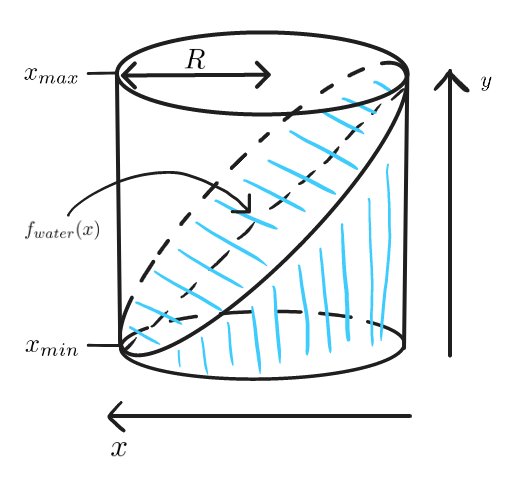
\includegraphics[width=.7\linewidth]{images/slanted_water.png}}
            \vspace{-10pt}
            \caption{Portion of water above $x_{min}$}
            \label{fig:slanted-water}
        \end{figure}
    \end{minipage}%
    \begin{minipage}{.5\linewidth}
        \begin{figure}[H]
            \centering
            \frame{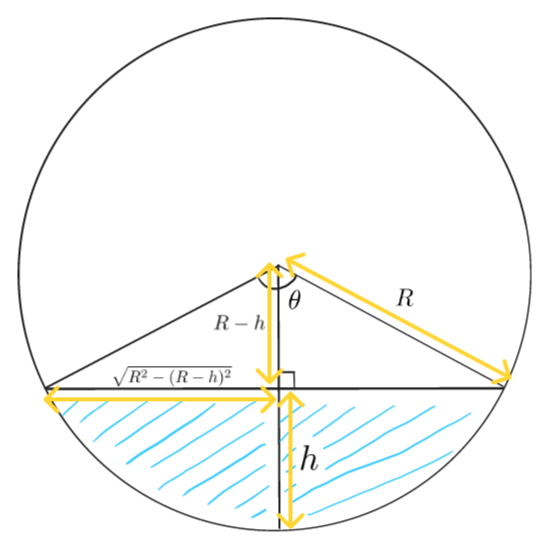
\includegraphics[width=.65\linewidth]{images/circle_segment.png}}
            \vspace{-10pt}
            \caption{A circular segment}
            \label{fig:circle-segment}
        \end{figure}
    \end{minipage}
    \vspace{2pt}

    The area of a circular segment is equal to the circular sector minus the triangle that is formed by the origin of the circle and the chord that separates the segment: ${A_{segment} = A_{sector} - A_{triangle}}$. The formulas for the areas of the sector and triangle can be derived separately, each as a function of $h$, and combined to get the formula for the area of a segment, as a function of $h$.

    \begin{minipage}{.4\linewidth}
        {\footnotesize\begin{align*}
            \cos{\left( \frac{\theta}{2} \right)} &= \frac{R - h}{R} \\
            \frac{\theta}{2} &= \arccos{\left( \frac{R - h}{R} \right)} \\
            \theta &= 2 \arccos{\left( \frac{R - h}{R} \right)} \numberthis{\label{eq:sector-theta}}
        \end{align*}}
    \end{minipage}%
    \begin{minipage}{.6\linewidth}
        {\footnotesize\begin{align*}
            A_{sector}(h) &= \pi R^2 \cdot \frac{\theta}{2\pi} \\
            \eqref{eq:sector-theta} \rightarrow A_{sector}(h) &= \pi R^2 \cdot \frac{2 \arccos{\left( \frac{R - h}{R} \right)}}{2\pi} \\
            &= R^2 \arccos{\left( \frac{R - h}{R} \right)} \\
            A_{sector}(h) &= R^2 \arccos{\left( 1 - \frac{h}{R} \right)}
        \end{align*}}
    \end{minipage}
    \vspace{2pt}

    Half of the triangle has height $R - h$ and hypotenuse $R$. Therefore, according to Pythagorean's Theorem, the base of half the triangle would be $\sqrt{R^2 - (R - h)^2}$. Combing both halves gives the total base length of the triangle to be $2 \sqrt{R^2 - (R - h)^2}$.
    {\footnotesize\begin{align*}
        A_{triangle}(h) &= \frac{\overbrace{(R - h)}^{\text{height}} \cdot \overbrace{2 \sqrt{R^2 - (R - h)^2}}^{\text{base}}}{2} \\
        A_{triangle}(h) &= (R - h) \cdot \sqrt{R^2 - (R - h)^2}
    \end{align*}}

    Combing these formulas gets the function $A_{segment}(h)$, where $R$ is the radius of the walls of the can, and with domain $\{ h \in \mathbb{R}, \, 0 \le h \le 2R \}$:
    {\footnotesize\begin{align*}
        A_{segment}(h) &= A_{sector}(h) - A_{triangle}(h) \\
        A_{segment}(h) &= R^2 \arccos{\left( 1 - \frac{h}{R} \right)} - (R - h) \cdot \sqrt{R^2 - (R - h)^2}
    \end{align*}}

    The height of the water at a point $x$ is the distance between the curve $f_{water}(x)$ and the bottom wall of the can. Because the can is symmetrical across the $x$ axis, the bottom wall of the can is the negative of the top wall of the can, $-f_5(x)$. Hence, the height of the water at a point $x$ is the difference between curves $f_{water}(x)$ and $-f_5(x)$. The function for height is ${h(x) = f_{water}(x) - (-f_5(x)) = f_{water}(x) + R}$.

    \begin{wrapfigure}{r}{.45\textwidth}
        \centering
        \frame{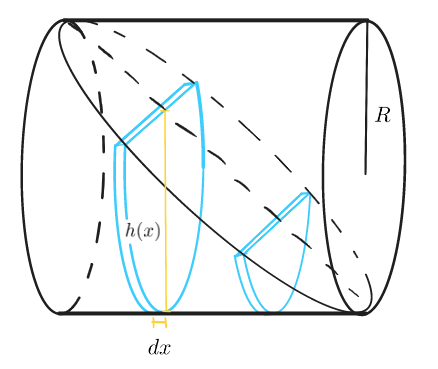
\includegraphics[width=.8\linewidth]{images/water_segments.png}}
        \vspace{-10pt}
        \caption{Slices along the $x$-axis of the can}
        \label{fig:water-segments}
    \end{wrapfigure}

    The volume of this portion of water can be split up into an infinite number of thin slices, with base area equal to $A_{segment}(h(x))$ and width $dx$, as visualized by the blue sections in Figure \ref{fig:water-segments}. The volume of one of these slices is its base multiplied by its width, so $dV = A_{segment}(h(x)) \, dx$. This value is expanded using $R = 32.35$ as follows:

    {\footnotesize\begin{align*}
        dV &= A_{segment}(h(x)) \, dx \\
        &= A_{segment}(f_{water}(x) + R) \, dx \\
        &= A_{segment}(-x + b + R) \, dx \\
        &= R^2 \arccos{\left( 1 - \frac{-x + b + R}{R} \right)} - (R - (-x + b + R)) \cdot \sqrt{R^2 - (R - (-x + b + R))^2} \, dx \\
        &= R^2 \arccos{\left( \frac{x - b}{R} \right)} - (x - b) \cdot \sqrt{R^2 - (x - b)^2} \, dx \\
        &= (32.35)^2 \arccos{\left( \frac{x - b}{32.35} \right)} - (x - b) \cdot \sqrt{(32.35)^2 - (x - b)^2} \, dx \\
        dV &= 1046.52 \arccos{\left( \frac{x - b}{32.35} \right)} - (x - b) \cdot \sqrt{1046.52 - (x - b)^2} \, dx
    \end{align*}}

    Substituting this value into equation \eqref{eq:CM-integral} with $a_i = x_{min}$ and $b_i = x_{max}$ gives:
    {\footnotesize\begin{align*}
        \overline{x} &= \frac{\int_{x_{min}}^{x_{max}} x dV}{V} \\
        &= \frac{\int_{x_{min}}^{x_{max}} x dV}{\int_{x_{min}}^{x_{max}} dV} \\
        \overline{x} &= \frac{\int_{x_{min}}^{x_{max}} x \left( 1046.52 \arccos{\left( \frac{x - b}{32.35} \right)} - (x - b) \cdot \sqrt{1046.52 - (x - b)^2} \right) \, dx}{\int_{x_{min}}^{x_{max}} 1046.52 \arccos{\left( \frac{x - b}{32.35} \right)} - (x - b) \cdot \sqrt{1046.52 - (x - b)^2} \, dx} \numberthis{\label{eq:water-top-vol}} \\
    \end{align*}}
    \vspace{-50pt}

    \begin{wrapfigure}{r}{.25\linewidth}
        \vspace{-25pt}
        {\footnotesize\begin{align*}
            \overline{x} &= \frac{423.19 \pi (80b - 647)}{33854.92 \pi} \\
            \overline{x} &\approx (b - 8.09) \mathrm{mm}
        \end{align*}}
    \end{wrapfigure}

    The definite integrals are solved separately using a website called Integral Calculator, with ${x_{min} = b - 32.35}$ and $x_{max} = b + 32.35$. The result is shown to the right.

    Once again, I noticed that the denominator of the right-hand side in equation \eqref{eq:water-top-vol} is equal to the volume of this portion of water, $V_{wt}$. For the purpose of efficiency, the definite integral was solved once again using the Integral Calculator.
    {\footnotesize\begin{align*}
        V_{wt} &= \int_{x_{min}}^{x_{max}} 1046.52 \arccos{\left( \frac{x - b}{32.35} \right)} - (x - b) \cdot \sqrt{1046.52 - (x - b)^2} \, dx \\
        V_{wt} &= (107443.3 \pi) \mathrm{mm}^3
    \end{align*}}

    \begin{wrapfigure}[3]{r}{.25\linewidth}
        \vspace{-30pt}
        {\footnotesize\begin{align*}
            y &= -x + b \\
            x &= b - y \\
            f^{-1}_{water}(y) &= b - y
        \end{align*}}
    \end{wrapfigure}

    The next step is to solve for $\overline{y}$ for this volume of water. First, the function for the surface of the water needs to be re-expressed as a function of $y$. This is done by taking the inverse of $f_{water}(x)$, shown to the right.

    \begin{wrapfigure}{l}{.4\textwidth}
        \centering
        \frame{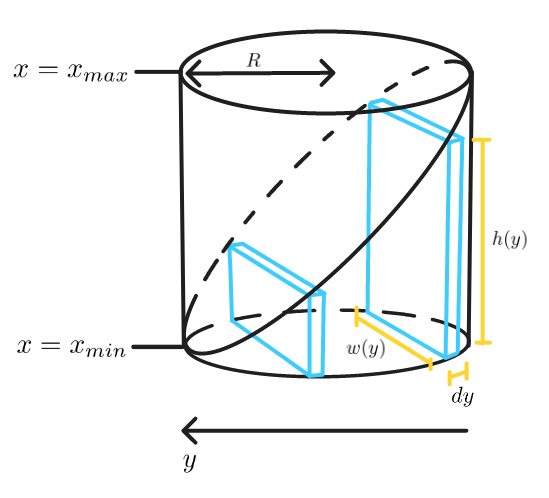
\includegraphics[width=.8\linewidth]{images/water_prisms_y.png}}
        \vspace{-10pt}
        \caption{Slices of water in the $y$-axis}
        \label{fig:water-prisms-y}
    \end{wrapfigure}

    To find $\overline{y}$ for this section of water, it is split up into an infinite number of thin slices, along the $y$-axis. This time, each slice is a rectangular prism, with height $h(y)$, width $w(y)$ and depth $dy$, as seen in Figure \ref{fig:water-prisms-y}. The height of each prism is the difference between $f^{-1}_{water}(y)$ and $x_{min}$, so ${h(y) = f^{-1}_{water}(y) - x_{min}}$. The width of each prism is the cylinder's circular base's chord's length perpendicular to the $y$-axis. Therefore, by Pythagorean's Theorem, ${w(y) = 2\sqrt{R^2 - |y|^2} = 2\sqrt{R^2 - y^2}}$. Altogether, the volume of each prism is:

    \vspace{-30pt}
    {\footnotesize\begin{align*}
        dV &= w(y) \cdot h(y) \cdot dy \\
        &= 2 \sqrt{R^2 - y^2} \cdot (f^{-1}_{water}(y) - x_{min}) \, dy \\
        &= 2 \sqrt{R^2 - y^2} \cdot \left( (b - y) - (b - R) \right) \, dy \\
        dV &= 2 (R - y) \sqrt{R^2 - y^2} \, dy
    \end{align*}}

    \begin{wrapfigure}[6]{r}{.33\linewidth}
        \vspace{-20pt}
        {\footnotesize\begin{align*}
            \overline{y} &= \frac{\int_{-R}^R y dV}{V} \\
            &= \frac{\int_{-R}^R y \cdot 2 (R - y) \sqrt{R^2 - y^2} \, dy}{V} \\
            &= \frac{-\frac{\pi R^4}{4}}{V} \\
            &= \frac{-\frac{\pi (32.35)^4}{4}}{107443.33} \\
            \overline{y} &\approx -8.01 \mathrm{mm}
        \end{align*}}
    \end{wrapfigure}

    Substituting this into an analogous equation of equation \eqref{eq:CM-integral} in terms of $y$, gives $\overline{y}$ for this volume of water. The limits for the definite integral are $\pm R$, and is solved using an online calculator. The total volume $V$ is the same as before, with ${V_{wt} = 107443.33 \mathrm{mm}^3}$. This process is shown to the right.

    This value makes sense as the $\overline{y}$ is slightly negative, reflecting the fact that there is more water underneath the $x$-axis. The value of $-8.01$ is also only about a quarter of the way to the bottom wall of the can with value $-R = -32.35$, meaning that the CM is closer to the middle of the can than its edge. To summarize, the CM's and total volumes of each portion of the can with water in each axis are listed in Table \ref{tab:cm-summary}.

    \begin{table}[H]
        \scriptsize
        \renewcommand{\arraystretch}{0.9}
        \centering
        \caption{Summary of the CM's and volumes}
        \vspace{-8pt}
        \begin{tabular}{|c|c|c|c|c|}
            \hline
            Portion & $\overline{x} (\mathrm{mm})$ & $\overline{y} (\mathrm{mm})$ & $\overline{z} (\mathrm{mm})$ & $V (\mathrm{mm}^3)$ \\
            \hline \hline
            Empty can & $48.74$ & $0$ & $0$ & $4314.30$ \\
            \hline
            Water at bottom of can & $\frac{0.5b^2 - 32.35b + 490.35}{b - 40.01}$ & $0$ & $0$ & $3287.74b - 131530.17$ \\
            \hline
            Water with slanted surface & $b - 8.09$ & $-8.01$ & $0$ & $107443.33$ \\
            \hline
        \end{tabular}
        \label{tab:cm-summary}
    \end{table}
    \vspace{-10pt}

    While it is true that the densities of materials change with temperature, the change is minimal. The room temperature of which this experiment is conducted in is unlikely to fluctuate anywhere close enough to affect the density of these materials and alter the results of this exploration (Talat; USGS). Therefore, the change in density due to temperature can safely be deemed as insignificant. To find the CM of the entire system, formula \eqref{eq:CM-density} can be used alongside the values from Table \ref{tab:cm-summary}. For the purpose of these calculations, subscript $c$ will refer to the can, $wb$ the bottom portion of water, and $wt$ the top portion of water. The CM in the $z$-axis will be $0$ because the $\overline{z}$ of each individual portion is $0$. All other units will cancel out in the end, leaving each component of the CM in millimeters. This will leave the CMs of the can in each axis in terms of $b$, and they can therefore be expressed as a function in terms of $b$.

    {\footnotesize\begin{align*}
        \overline{x} &= \frac{\sum_i \overline{x_i} \rho_i V_i}{\sum_i \rho_i V_i} \\
        &= \frac{\overline{x_c} \rho_{a} V_c + \overline{x_{wb}} \rho_{w} V_{wb} + \overline{x_{wt}} \rho_{w} V_{wt}}{\rho_{a} V_c + \rho_{w} V_{wb} + \rho_{w} V_{wt}} \\
        &= \frac{48.74 \cdot 0.0027 \cdot 4314.30 + \left( \frac{0.5b^2 - 32.35b + 490.35}{b - 40.01} \right) \cdot 0.001 \cdot (3287.74b - 131530.17) + (b - 8.09) \cdot 0.001 \cdot 107443.33}{0.0027 \cdot 4314.30 + 0.001 \cdot (3287.74b - 131530.17) + 0.001 \cdot 107443.33} \\
        \overline{x}(b) &\approx \frac{0.5b^3 - 19.67b^2 + 385.33b - 15948.4}{b^2 - 43.79b + 151.36} \\[12pt]
        \overline{y} &= \frac{\sum_i \overline{y_i} \rho_i V_i}{\sum_i \rho_i V_i} \\
        &= \frac{\overline{y_c} \rho_{a} V_c + \overline{y_{wb}} \rho_{w} V_{wb} + \overline{y_{wt}} \rho_{w} V_{wt}}{\rho_{a} V_c + \rho_{w} V_{wb} + \rho_{w} V_{wt}} \\
        &= \frac{0 \cdot 0.0027 \cdot 4314.30 + 0 \cdot 0.001 \cdot (3287.74b - 131530.17) + (-8.01) \cdot 0.001 \cdot 107443.33}{0.0027 \cdot 4314.30 + 0.001 \cdot (3287.74b - 131530.17) + 0.001 \cdot 107443.33} \\
        \overline{y}(b) &\approx -\frac{261.77}{b - 3.78}
    \end{align*}}

    \begin{wrapfigure}{r}{.35\textwidth}
        \centering
        \frame{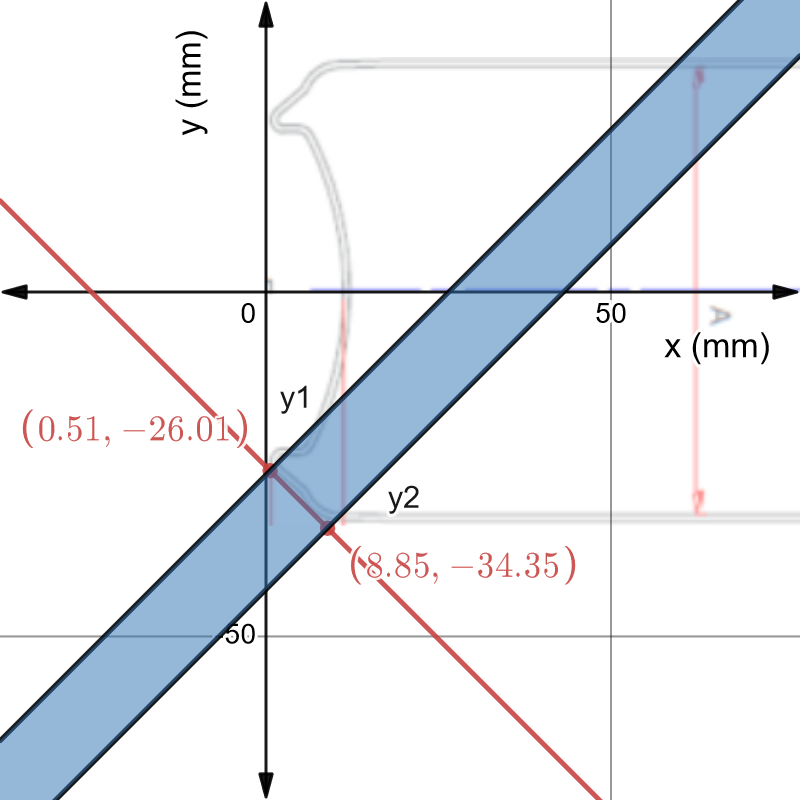
\includegraphics[width=.9\linewidth]{images/floor.png}}
        \caption{Region for possible CMs}
        \label{fig:floor-points}
    \end{wrapfigure}

    In order to find the range of values of $b$ for which the can balances on its edge, I first need to find the left and right-most points for which the can touches the ground when on an angle. I found these two points by analysing where the image of the can touched line the represented the ground. The two points are at $p_1 = (0.51, -26.01)$ and $p_2 = (8.85, -34.35)$, as seen in Figure \ref{fig:floor-points}. The slope of the floor is derived to be: $m = \frac{-34.35 + 26.01}{8.85 - 0.51} = -1$. This value makes sense as the floor is parallel to the surface of the water, and this is the same slope as $f_{water}(x)$.

    For an object to be able to balance, its CM must either be directly above or in between two points that touch the floor. The CM is above the point on the floor, forming a perpendicular line to the floor itself. Therefore, the furthest ends of the CM for which the object will still balance are dictated by the two lines, $y_1$ and $y_2$ (Figure \ref{fig:floor-points}), which are perpendicular to the floor and respectively pass through $p_1$ and $p_2$. The slopes of these tangent lines are the negative reciprocal of the floor line, hence the slopes of $y_1$ and $y_2$ are $1$. Given this slope, the parent equation for these two lines are therefore $y = x + k$, where $k$ is the $y$-intercept. Solving for each $k$ by substituting in $p_1$ and $p_2$ into $y_1$ and $y_2$, respectively, yields $y_1 = x - 26.52$ and $y_2 = x - 43.2$.

    The can will balance if its CM is anywhere inside the region between $y_1$ and $y_2$, shown in blue in Figure \ref{fig:floor-points}. This region can be expressed as the inequality $y_1 \ge y \ge y_2$. I split this inequality into two separate ones, $y_1 \ge y$ and $y \ge y_2$, then re-expressed them in terms of $b$ by substituting in $\overline{x}(b)$ for $x$ and $\overline{y}(b)$ for $y$. I used Wolfram Alpha to solve the inequality and find the range of values of $b$ for which the can will balance.

    {\footnotesize\begin{align*}
        y_1 &\ge y \\
        y &\le x - 26.52 \\
        \overline{y}(b) &\le \overline{x}(b) - 26.52 \\
        -\frac{261.77}{b - 3.78} &\le \frac{0.5b^3 - 19.67b^2 + 385.33b - 15948.4}{b^2 - 43.79b + 151.36} - 26.52 \numberthis{\label{eq:inequality-1}} \\[10pt]
        y &\ge y_2 \\
        y &\ge x - 43.2 \\
        \overline{y}(b) &\ge \overline{x}(b) - 43.2 \\
        -\frac{261.77}{b - 3.78} &\ge \frac{0.5b^3 - 19.67b^2 + 385.33b - 15948.4}{b^2 - 43.79b + 151.36} - 43.2 \numberthis{\label{eq:inequality-2}}
    \end{align*}}

    Inequality \eqref{eq:inequality-1} gives approximately $b > 3.78$, and inequality \eqref{eq:inequality-2} gives approximately $b < 3.78$ and $29.08 \le b \le 56.64$. Furthermore, I took into account the inequality for $b$ based on the assumption that $x_{min}$ does not go below a certain point, where $b \ge 44.85$. The range of $b$ values for which all three sets of inequalities covers is $44.85 \le b \le 56.64$. Note that there are two values of $b$ for which the numerator of either $\overline{x}(b)$ or $\overline{y}(b)$ would be $0$, making the inequality undefined. These are at $b \approx 3.78$ and $b \approx 40$, but neither are within the final range of possible $b$ values, so they are not taken into account.

    Finally, I converted the range of $b$ values to a range of possible volumes for which the can will balance. I combined the functions for the volumes of the bottom and top portions of water to get a function for the total volume of water in terms of $b$.
    {\footnotesize\begin{align*}
        V_{water}(b) &= V_{wb}(b) + V_{wt}(b) \\
        &= 3287.74b - 131530.17 + 107443.33 \\
        V_{water}(b) &= (3287.74b - 24086.84) \mathrm{mm}^3 \numberthis{\label{eq:total-volume}}
    \end{align*}}

    I substituted in the minimum and maximum values of $b$ to get the minimum and maximum volumes, respectively. Hence, $V_{water}(44.85) \approx 123368 \mathrm{mm}^3$ and $V_{water}(56.64) \approx 162131 \mathrm{mm}^3$. Converting these values to milliliters and rewriting as an inequality yields approximately $123 \mathrm{mL} \le V \le 162 \mathrm{mL}$. These numbers are rounded to the nearest whole number to match the precision of my scale. Therefore, given the restrictions of this exploration, a soda can will theoretically be able to stand on its edge if there is between $123 \mathrm{mL}$ and $162 \mathrm{mL}$ of water within it. In order to validate my calculations, I took a can and first filled it up with $123 \mathrm{mL}$ of water, and it was able to balance on its edge, thereby confirming the lower bound of my calculated range (Figure \ref{fig:scale-123}). However, I slowly poured out the water from the can bit by bit until the can was no longer able to balance. Through experimentation, I found out that the real lower bound for possible volume of water in the can was $65 \mathrm{mL}$ (Figure \ref{fig:scale-65}). This makes sense because I limited the domain of my calculations so that $x_{min} \ge 12.5$. Next, I tested out the upper bound of my calculated range. The can was also able to balance with $162 \mathrm{mL}$ (Figure \ref{fig:scale-162}). Further validating this calculation, when I added just $5 \mathrm{mL}$ more of water to have a total of $167 \mathrm{mL}$ of water in the can, it was no longer able to balance. Unfortunately, it was impossible to capture this result in a photo.

    \begin{figure}[H]
        \centering
        \begin{subfigure}{.3\textwidth}
            \centering
            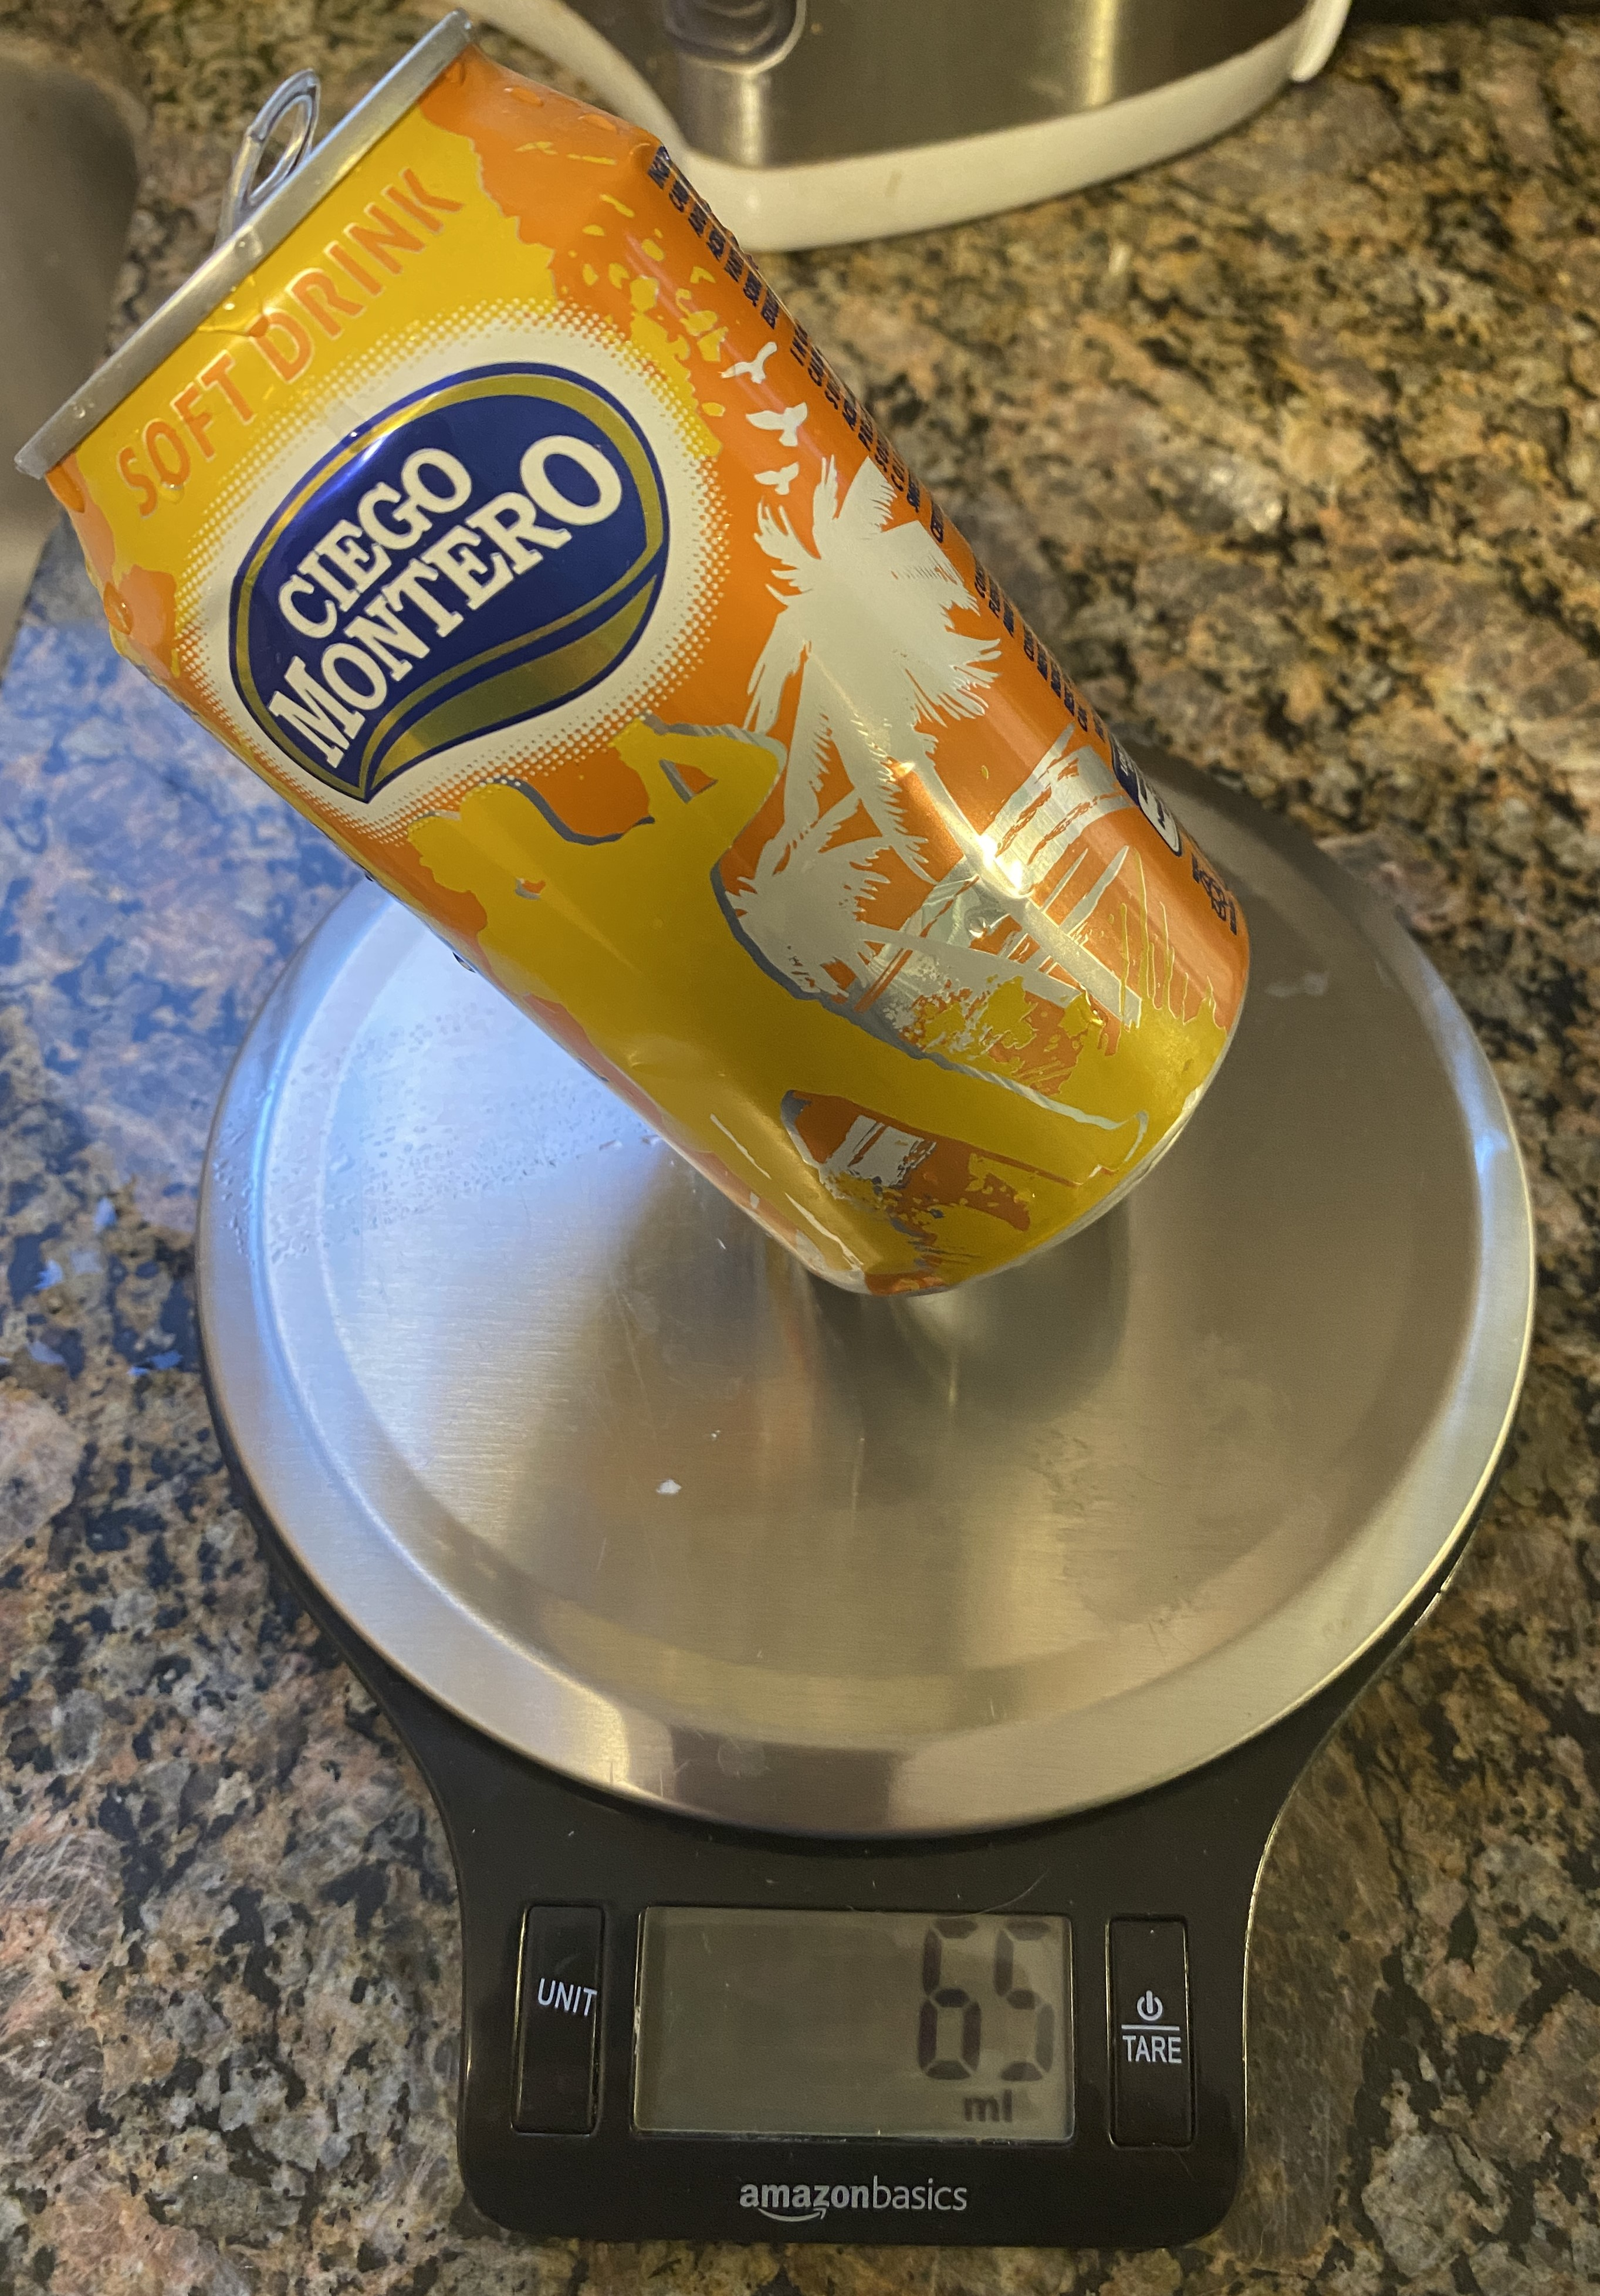
\includegraphics[width=.88\linewidth]{images/scale_65.JPG}
            \vspace{-8pt}
            \caption{$65 \mathrm{mL}$ of water}
            \label{fig:scale-65}
        \end{subfigure}
        \begin{subfigure}{.3\textwidth}
            \centering
            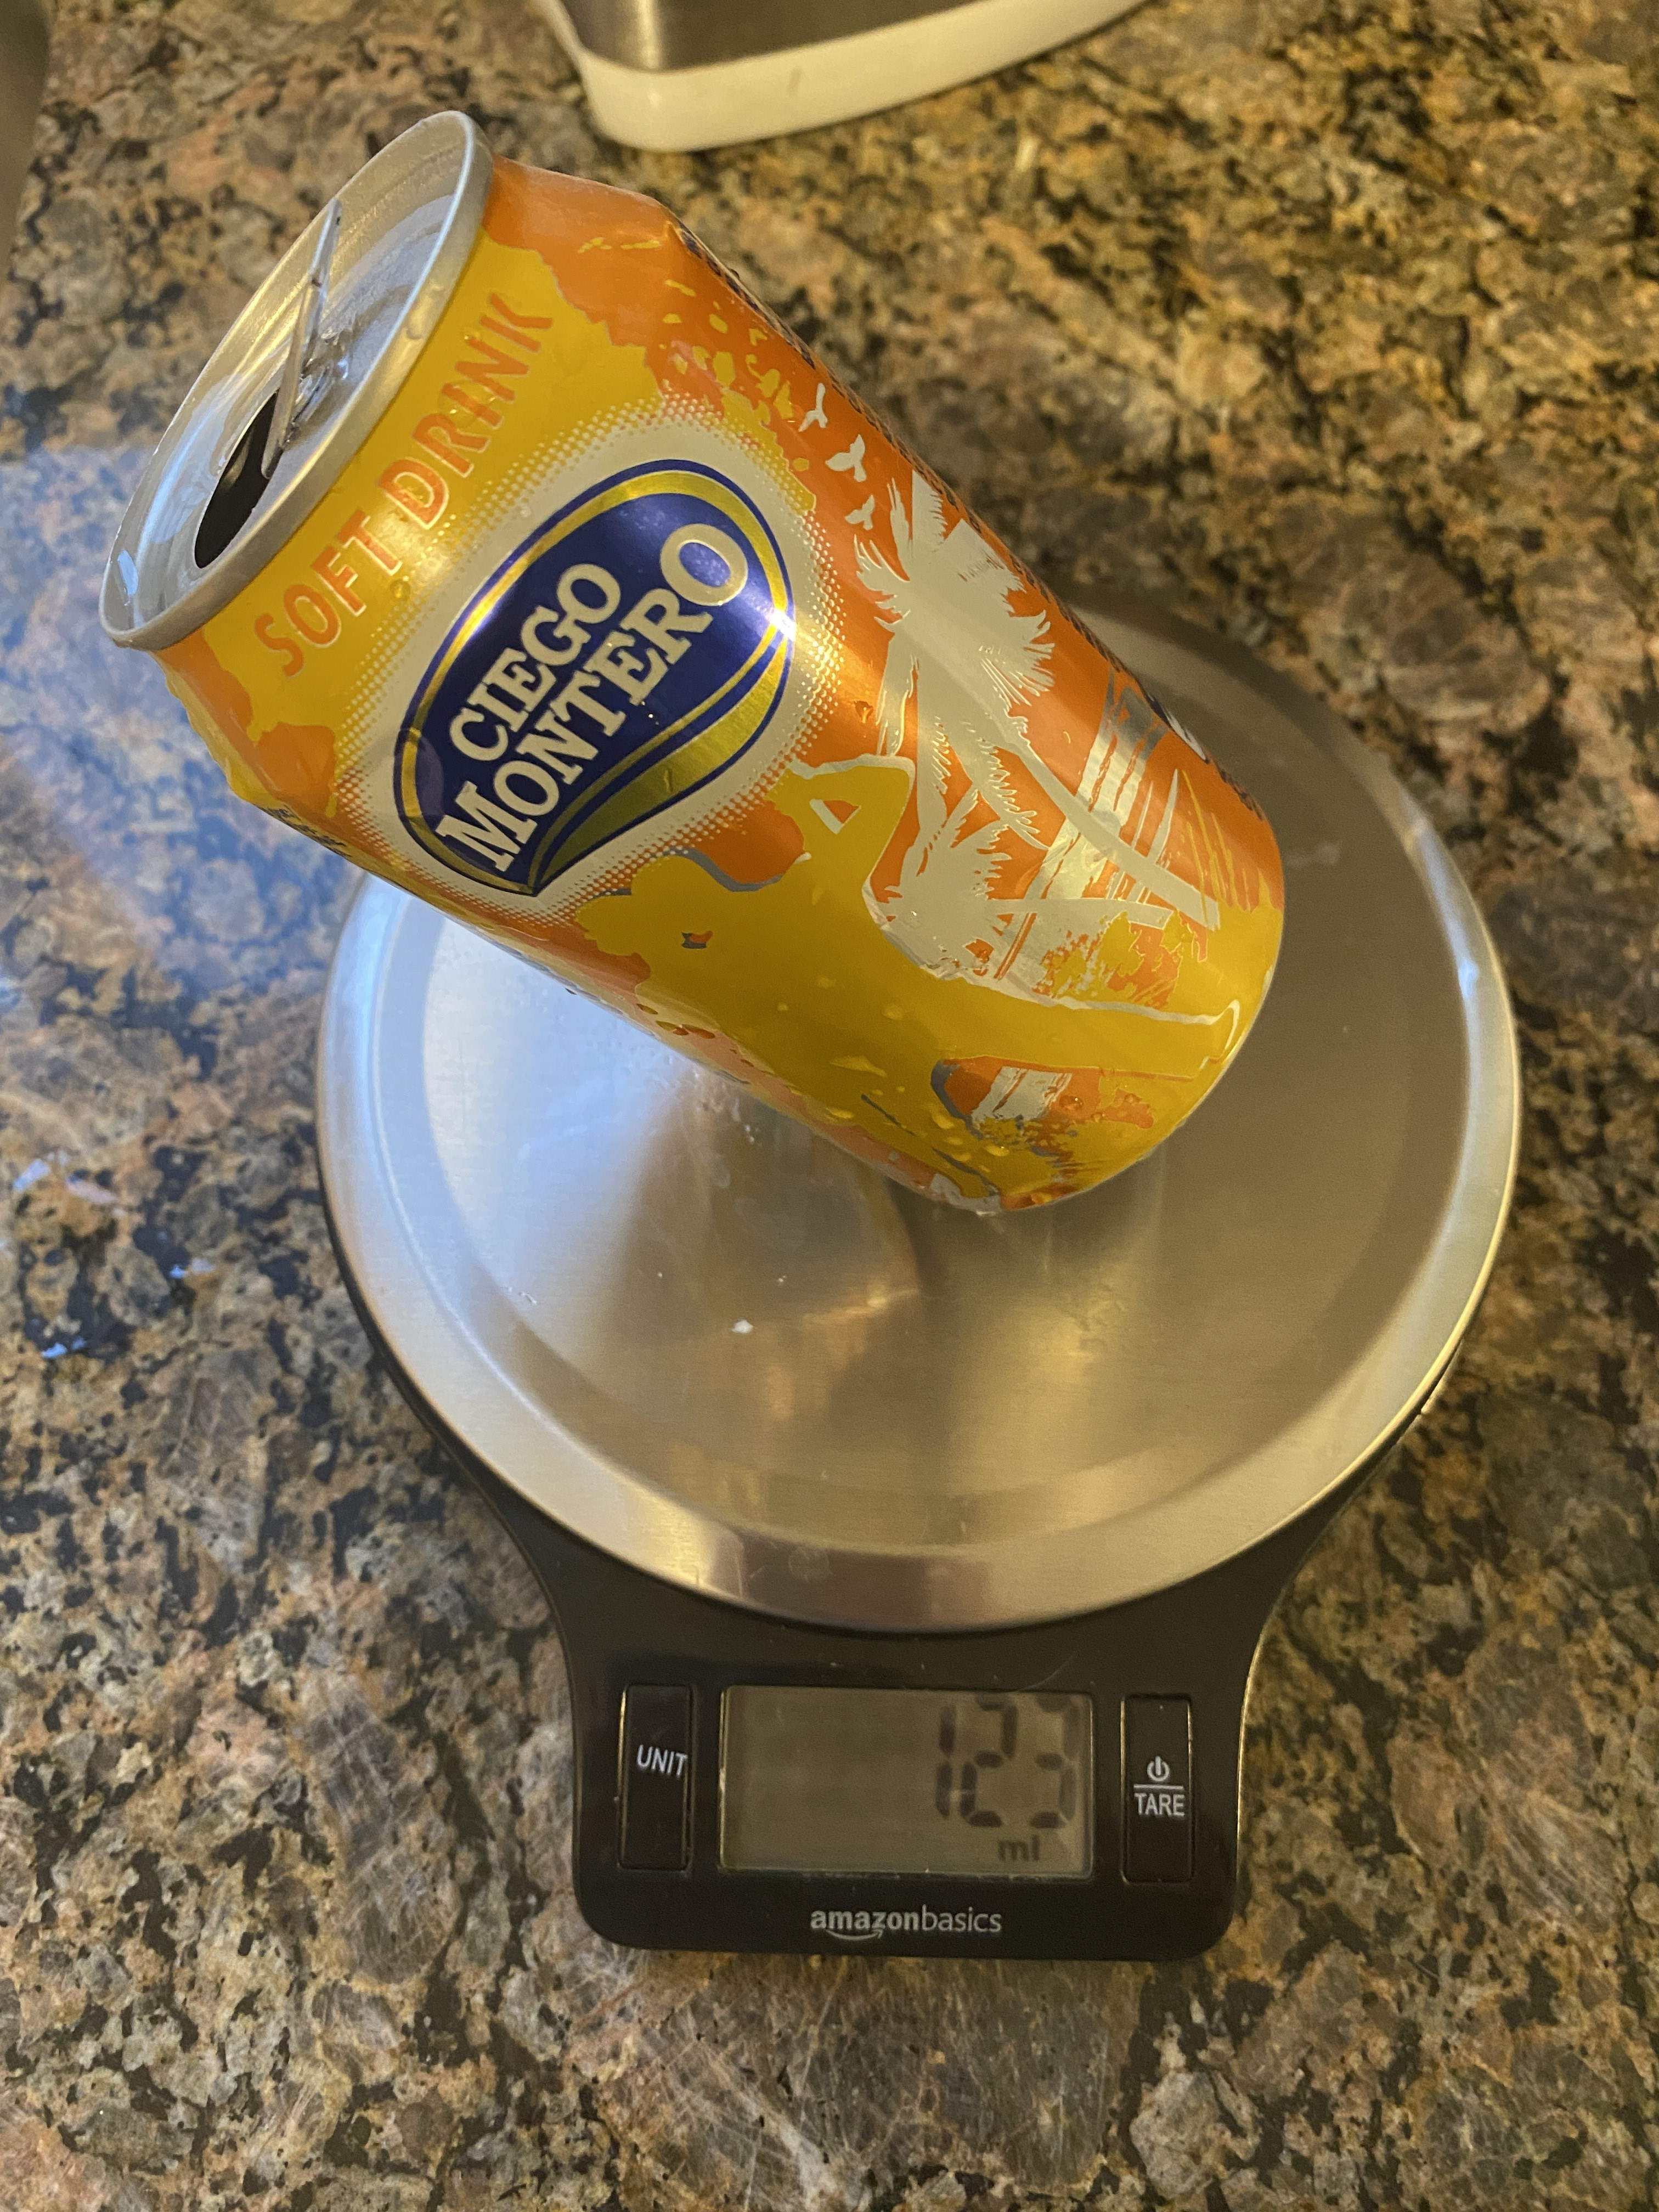
\includegraphics[width=.95\linewidth]{images/scale_123.JPG}
            \vspace{-8pt}
            \caption{$123 \mathrm{mL}$ of water}
            \label{fig:scale-123}
        \end{subfigure}
        \begin{subfigure}{.3\textwidth}
            \centering
            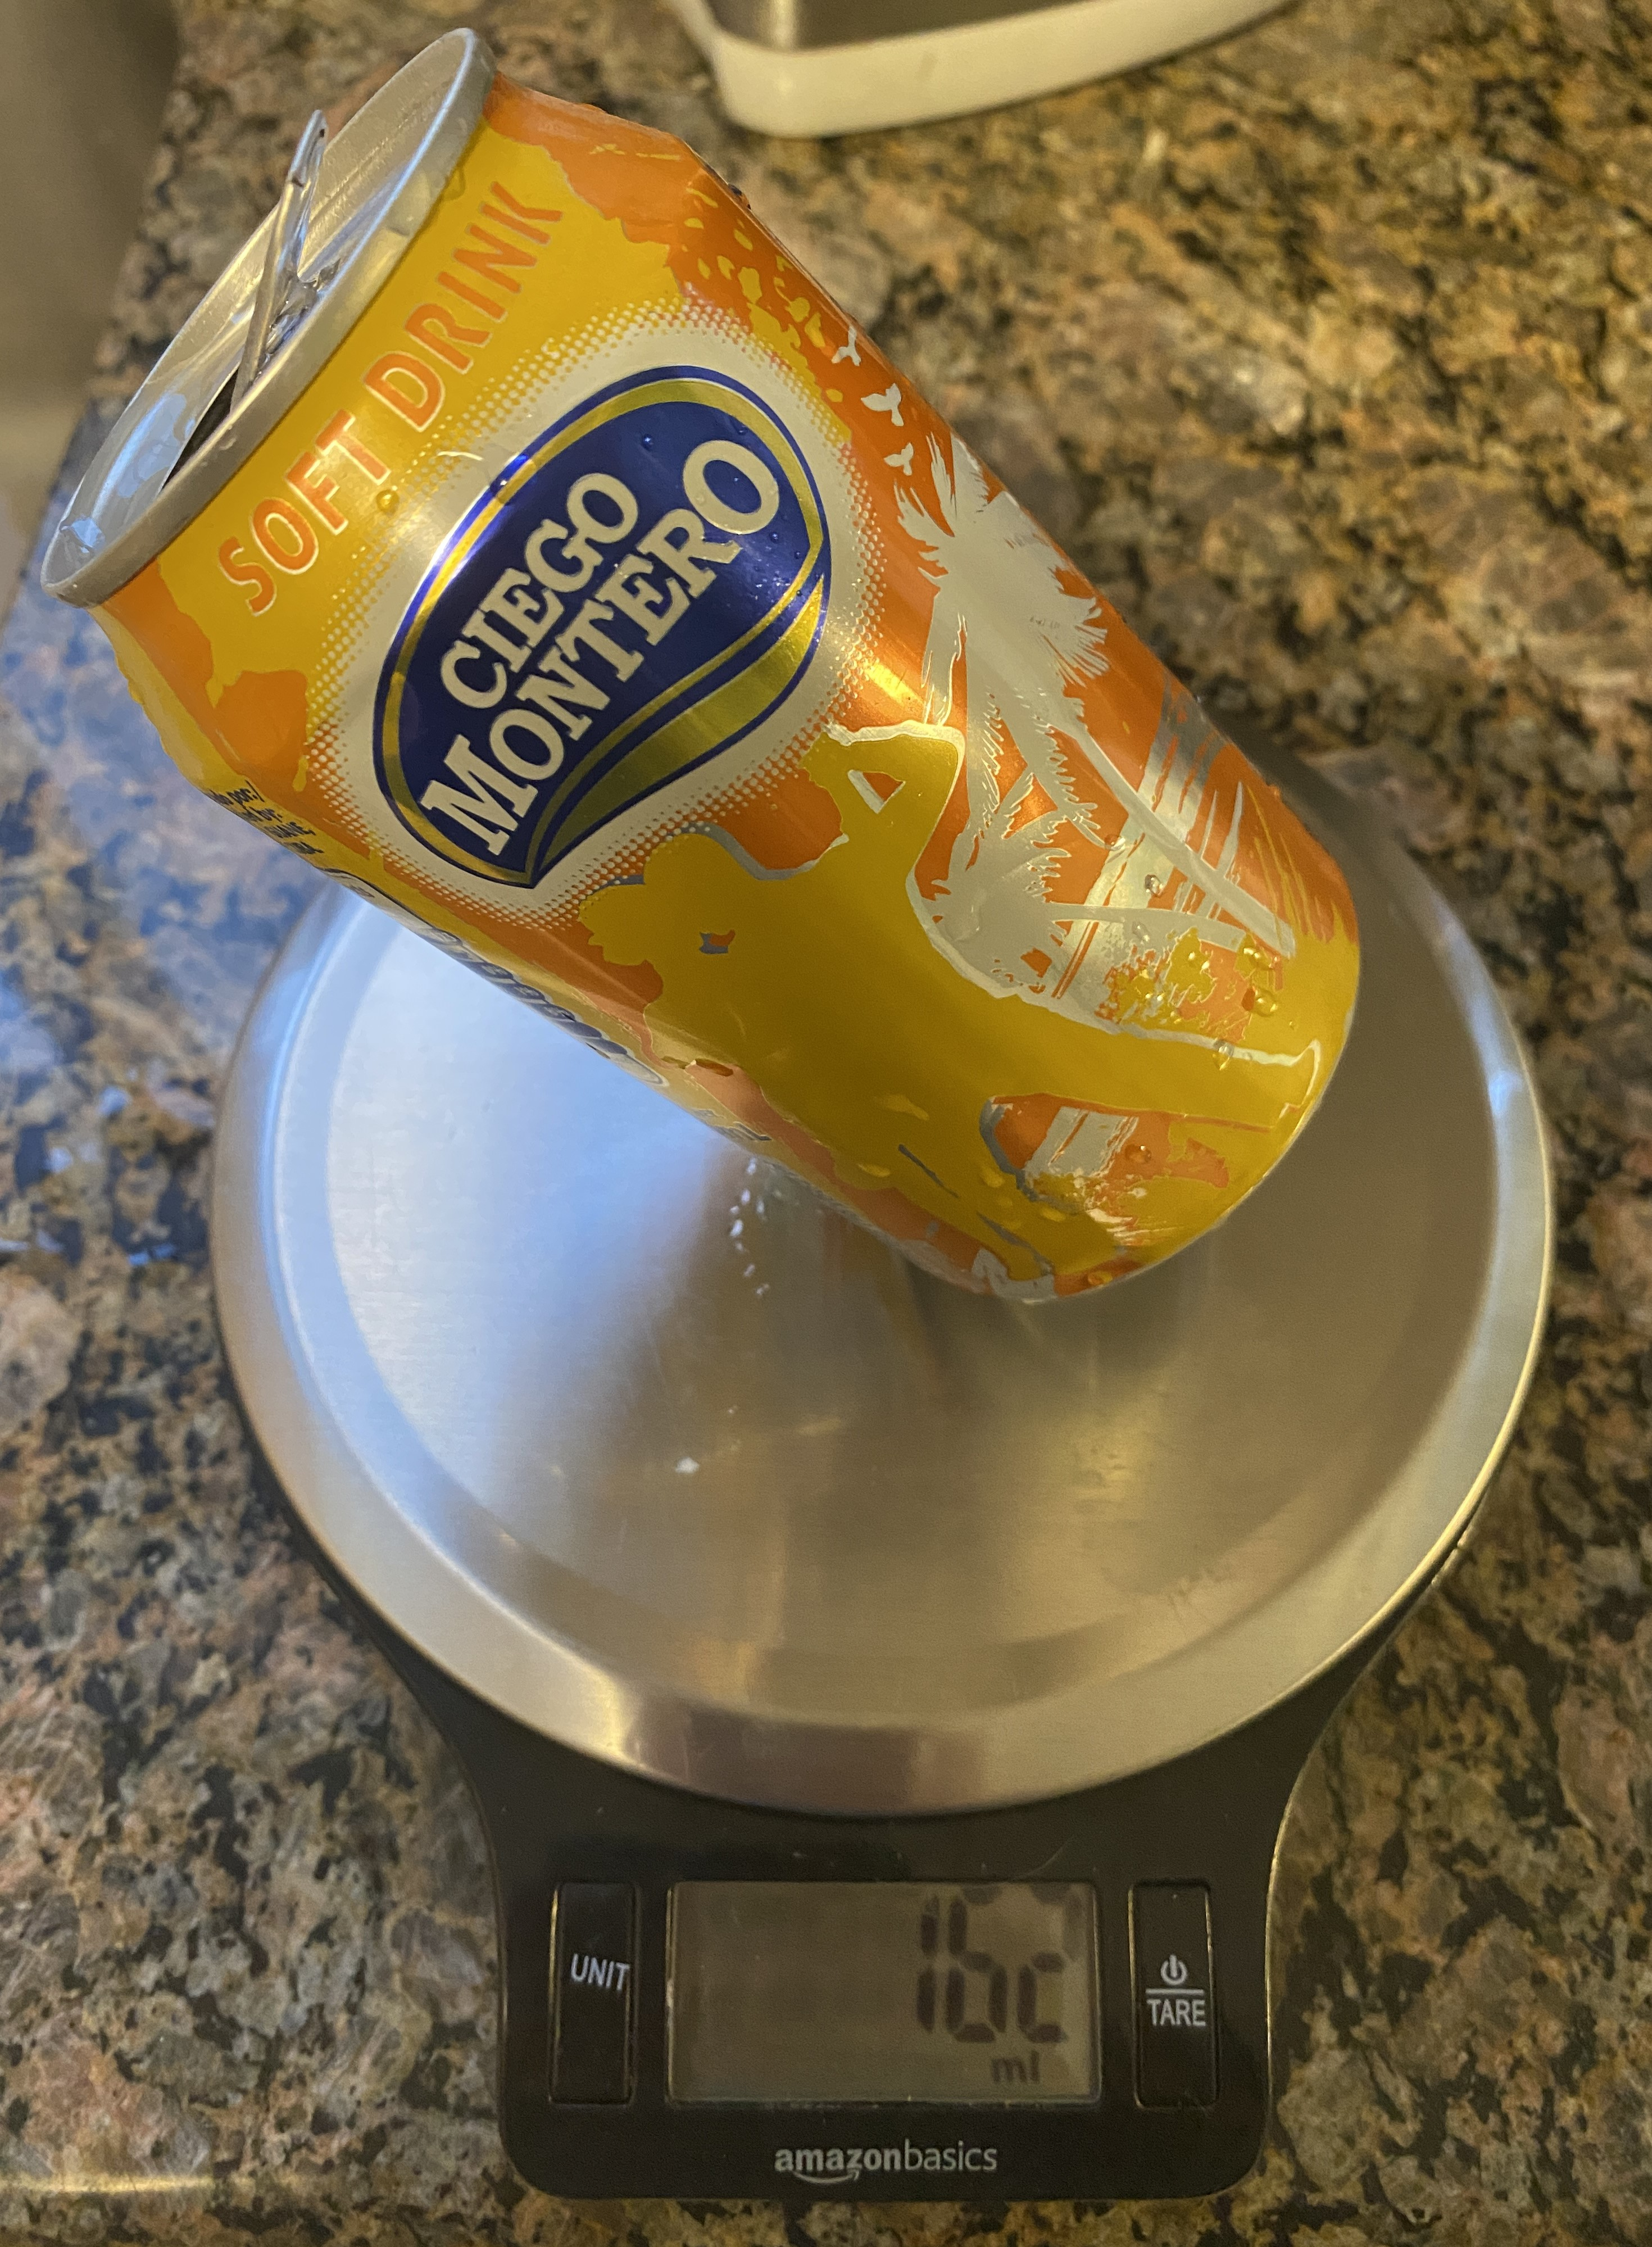
\includegraphics[width=.93\linewidth]{images/scale_162.JPG}
            \vspace{-8pt}
            \caption{$162 \mathrm{mL}$ of water}
            \label{fig:scale-162}
        \end{subfigure}
        \vspace{-10pt}
        \caption{Can balances with different volumes of water}
        \label{fig:scale}
    \end{figure}
    \vspace{-10pt}

    The strength of this exploration lies in the utilisation of Desmos to accurately model the can mathematically, and the use of integration to most accurately calculate the CMs of the entire can. However, the biggest limitation of this exploration is the assumption that the water will not go below the variable $x_{min}$, which effectively negated a whole range of possible volumes from the final calculation. Regardless, this exploration turned out to be successful in finding the amount of water needed in a can for it to be able to balance on its edge. Some possibilities for taking this idea further include finding the amount of soda, which has a lower density than water, needed for the can to balance, or how much water is needed for cans of different sizes.

    \newpage
    \renewcommand{\thepage}{} % dont number the bibliography page
    \nocite{can_ends}
    \nocite{helvetia_packaging}
    \nocite{isaac_physics}
    \nocite{moore_2021}
    \nocite{mulkins_2019}
    \nocite{talat_cans}
    \nocite{talat_density}
    \nocite{water_density}
    \printbibliography
\end{document}